%%%%%%%%%%%%%%%%%%%%%%%%%%%%%%%%%%%%%%%%%%%%%%%%%%%%%%%%%%%%
%%% ELIFE ARTICLE TEMPLATE
%%%%%%%%%%%%%%%%%%%%%%%%%%%%%%%%%%%%%%%%%%%%%%%%%%%%%%%%%%%%
%%% PREAMBLE 
\documentclass[9pt,lineno]{elife}

\usepackage[export]{adjustbox}
\usepackage{lscape}
\usepackage{afterpage}
\usepackage{hyperref}
\hypersetup{
    colorlinks=true,
    linkcolor=blue,
    filecolor=magenta,      
    urlcolor=cyan,
}

\newcommand{\sgcomment}[1]{\textcolor{blue}{SG: #1}}
\newcommand{\luke}[1]{\textcolor{blue}{Luke: #1}}
\newcommand{\todo}[1]{\textcolor{blue}{*#1*}}
\newcommand{\alex}[1]{\textcolor{red}{Alex: #1}}

%\newcommand{\qq}{m}

%%%%%%%%%%%%%%%%%%%%%%%%%%%%%%%%%%%%%%%%%%%%%%%%%%%%%%%%%%%%
%%% ARTICLE SETUP
%%%%%%%%%%%%%%%%%%%%%%%%%%%%%%%%%%%%%%%%%%%%%%%%%%%%%%%%%%%%
%\title{Legacy Data Confounds Modern Genomics Studies}
\title{Batch Effects in the 1000 Genomes Project Data Confound Modern Genomics Studies}

\author[1,2]{Luke Anderson-Trocm\'e}
\author[1,2]{Rick Farouni}
\author[1,2]{Mathieu Bourgey}
\author[3]{Fumihiko Matsuda}
\author[3]{Yoichiro Kamatani}
\author[1,2]{Simon Gravel}

\affil[1]{Department of Human Genetics, McGill University, Montreal, QC H3A 0G1, Canada}
\affil[2]{McGill University and Genome Quebec Innovation Centre, Montreal, QC H3A 0G1, Canada}
\affil[3]{Center for Genomic Medicine, Graduate School of Medicine, Kyoto University, Kyoto 606-8501, Japan}
\corr{simon.gravel@mcgill.ca}{SG}

%%%%%%%%%%%%%%%%%%%%%%%%%%%%%%%%%%%%%%%%%%%%%%%%%%%%%%%%%%%%
%%% ARTICLE START
%%%%%%%%%%%%%%%%%%%%%%%%%%%%%%%%%%%%%%%%%%%%%%%%%%%%%%%%%%%%

\begin{document}

\maketitle
\begin{abstract}
Recent reports have identified differences in the mutational spectra across human populations. While some of these reports have been replicated in other cohorts, most have been reported in the 1000 Genomes project data. While investigating an intriguing putative population stratification within the Japanese population, we identified a previously unreported batch effect leading to spurious mutation calls in the 1000 Genomes Project data and to the apparent population stratification. Because the 1000 Genomes data is used extensively, we find that the spurious calls also lead to incorrect imputation by leading imputation servers and suspicious GWAS associations. Lower-quality data from the early phases of the 1000 Genomes project thus contaminates modern studies in hidden ways, and a community effort may be required to remove or upgrade such legacy sequencing data from reference databases. 
\end{abstract}

\section{Introduction}
		
\subsection{Batch Effects in Aging Reference Cohort Data}			

The last 5 years have seen a drastic increase in the amount and quality of human genome sequence data. 
Reference cohorts such as the International HapMap Project \citep{HapMap2005}, the 1000 Genomes Project \citep{1000GenomesProjectConsortium2010,The1000GenomesProjectConsortium2012}, and the Simons Diversity project \citep{Mallick2016}, for example, have made thousands of genome sequences publicly available for population and medical genetic analyses. 
Many more genomes are available indirectly through servers providing imputation services \citep{HapMap2005} or summary statistics for variant frequency estimation \citep{Lek2016}.

Because of the extraordinary value of freely available data, this early data from the 1000 Genomes project (1kGP) is still widely used as a reference panel for imputation, allele frequency estimations and to answer a wide range of medical and evolutionary questions. 
However, the first sequenced genomes in the 1kGP, for example, were sequenced 10 years ago \citep{VanDijk2014}. Since then, sequencing platforms have rapidly improved. 
The second phase of the 1kGP implemented multiple technological and analytical improvements over its earlier phases \citep{The1000GenomesProjectConsortium2012}. 
This led to heterogeneous sample preparations and data quality for many of the samples included in the dataset.
This begs the question: when should we retire legacy reference data?

Even though it is intuitively clear that such batch effects have the potential to confound analyses, the usefulness and ubiquity of the 1kGP data make such issues particularly insidious.   
This raises the question of whether and how such legacy data should be included in contemporary analyses alongside more recent cohorts.
Here we point out how large and previously unreported batch effects in the early phases of the 1kGP still lead to incorrect genetic conclusions through population genetic analyses and indirect use through prominent imputation servers.


\subsection{Mutational Signatures}

Some mutagenic processes will affect different DNA motifs. 
Certain mutagens in tobacco smoke, for example, have been shown to preferentially bind to certain genomic motifs leading to an excess of G to T transversions \citep{Pfeifer2002,Pleasance2010}. 
Thus, exposure of populations to different mutational processes can be inferred by considering the DNA context of polymorphism in search of \textit{signatures} of different mutational processes \citep{Alexandrov2013,Shiraishi2015a}. 
Such genome wide mutational signatures have been used as diagnostic tools for cancers \citep{Alexandrov2013,Shiraishi2015a}.

While certain mutagens have very distinct mutational signatures, others are more subtle and require much larger datasets to identify because they tend to occur less frequently and with less genomic specificity \citep{Pleasance2010}.
Differences in mutational signatures across human populations have recently been reported.
In 2015, Harris reported 50\% more TCC ${\rightarrow}$ TTC mutations in European populations compared to African populations; this was replicated in a different cohort in 2017 \citep{Harris2015a, Harris2017a, Mathieson2017a}. 
Strong population enrichments of a mutational signature suggests important genetic or environmental differences in the history of each population \citep{Harris2015a, Harris2017a}. 
Harris and Pritchard further identified distinct mutational spectra across a range of populations, which were further examined in a recent publication by Aikens et al. \citep{Harris2017a,Aikens2018}.
 
 In particular, both studies  identified a heterogeneous mutational signature within 1000 Genomes Japanese individuals.
This heterogeneity is intriguing because differences in mutational signatures accumulate over many generations.
A systematic difference within the Japanese population would suggest sustained environmental or genetic differences across sub-populations within Japan with little to no gene flow.
We therefore decided to follow up on this observation, by using a newly sequenced dataset \sgcomment{description of cohort.}

While we were unable to reproduce the heterogeneity within the Japanese population, we could trace back the source of the discrepancy to a batch effect in the 1kGP data that we were not previously aware of.
We also found that this batch effect led to spurious results in a additional recent publications as a consequence of biased imputation.


The results section is organized as follows.
First, we explore the mutational signal found in the 1kGP Japanese population and methods by which we can identify this technical artifact.
Next, we expand our analysis to the other populations in the 1kGP and identify lists of SNPs whose validity is highly debatable.
Finally, we investigate how these SNPs have impacted modern genomics analyses. 
We report that major imputation servers impute the dubious SNPs. 
We also identify two publications that report such SNPs as genome-wide significant or nearly significant hits.   

\begin{figure}
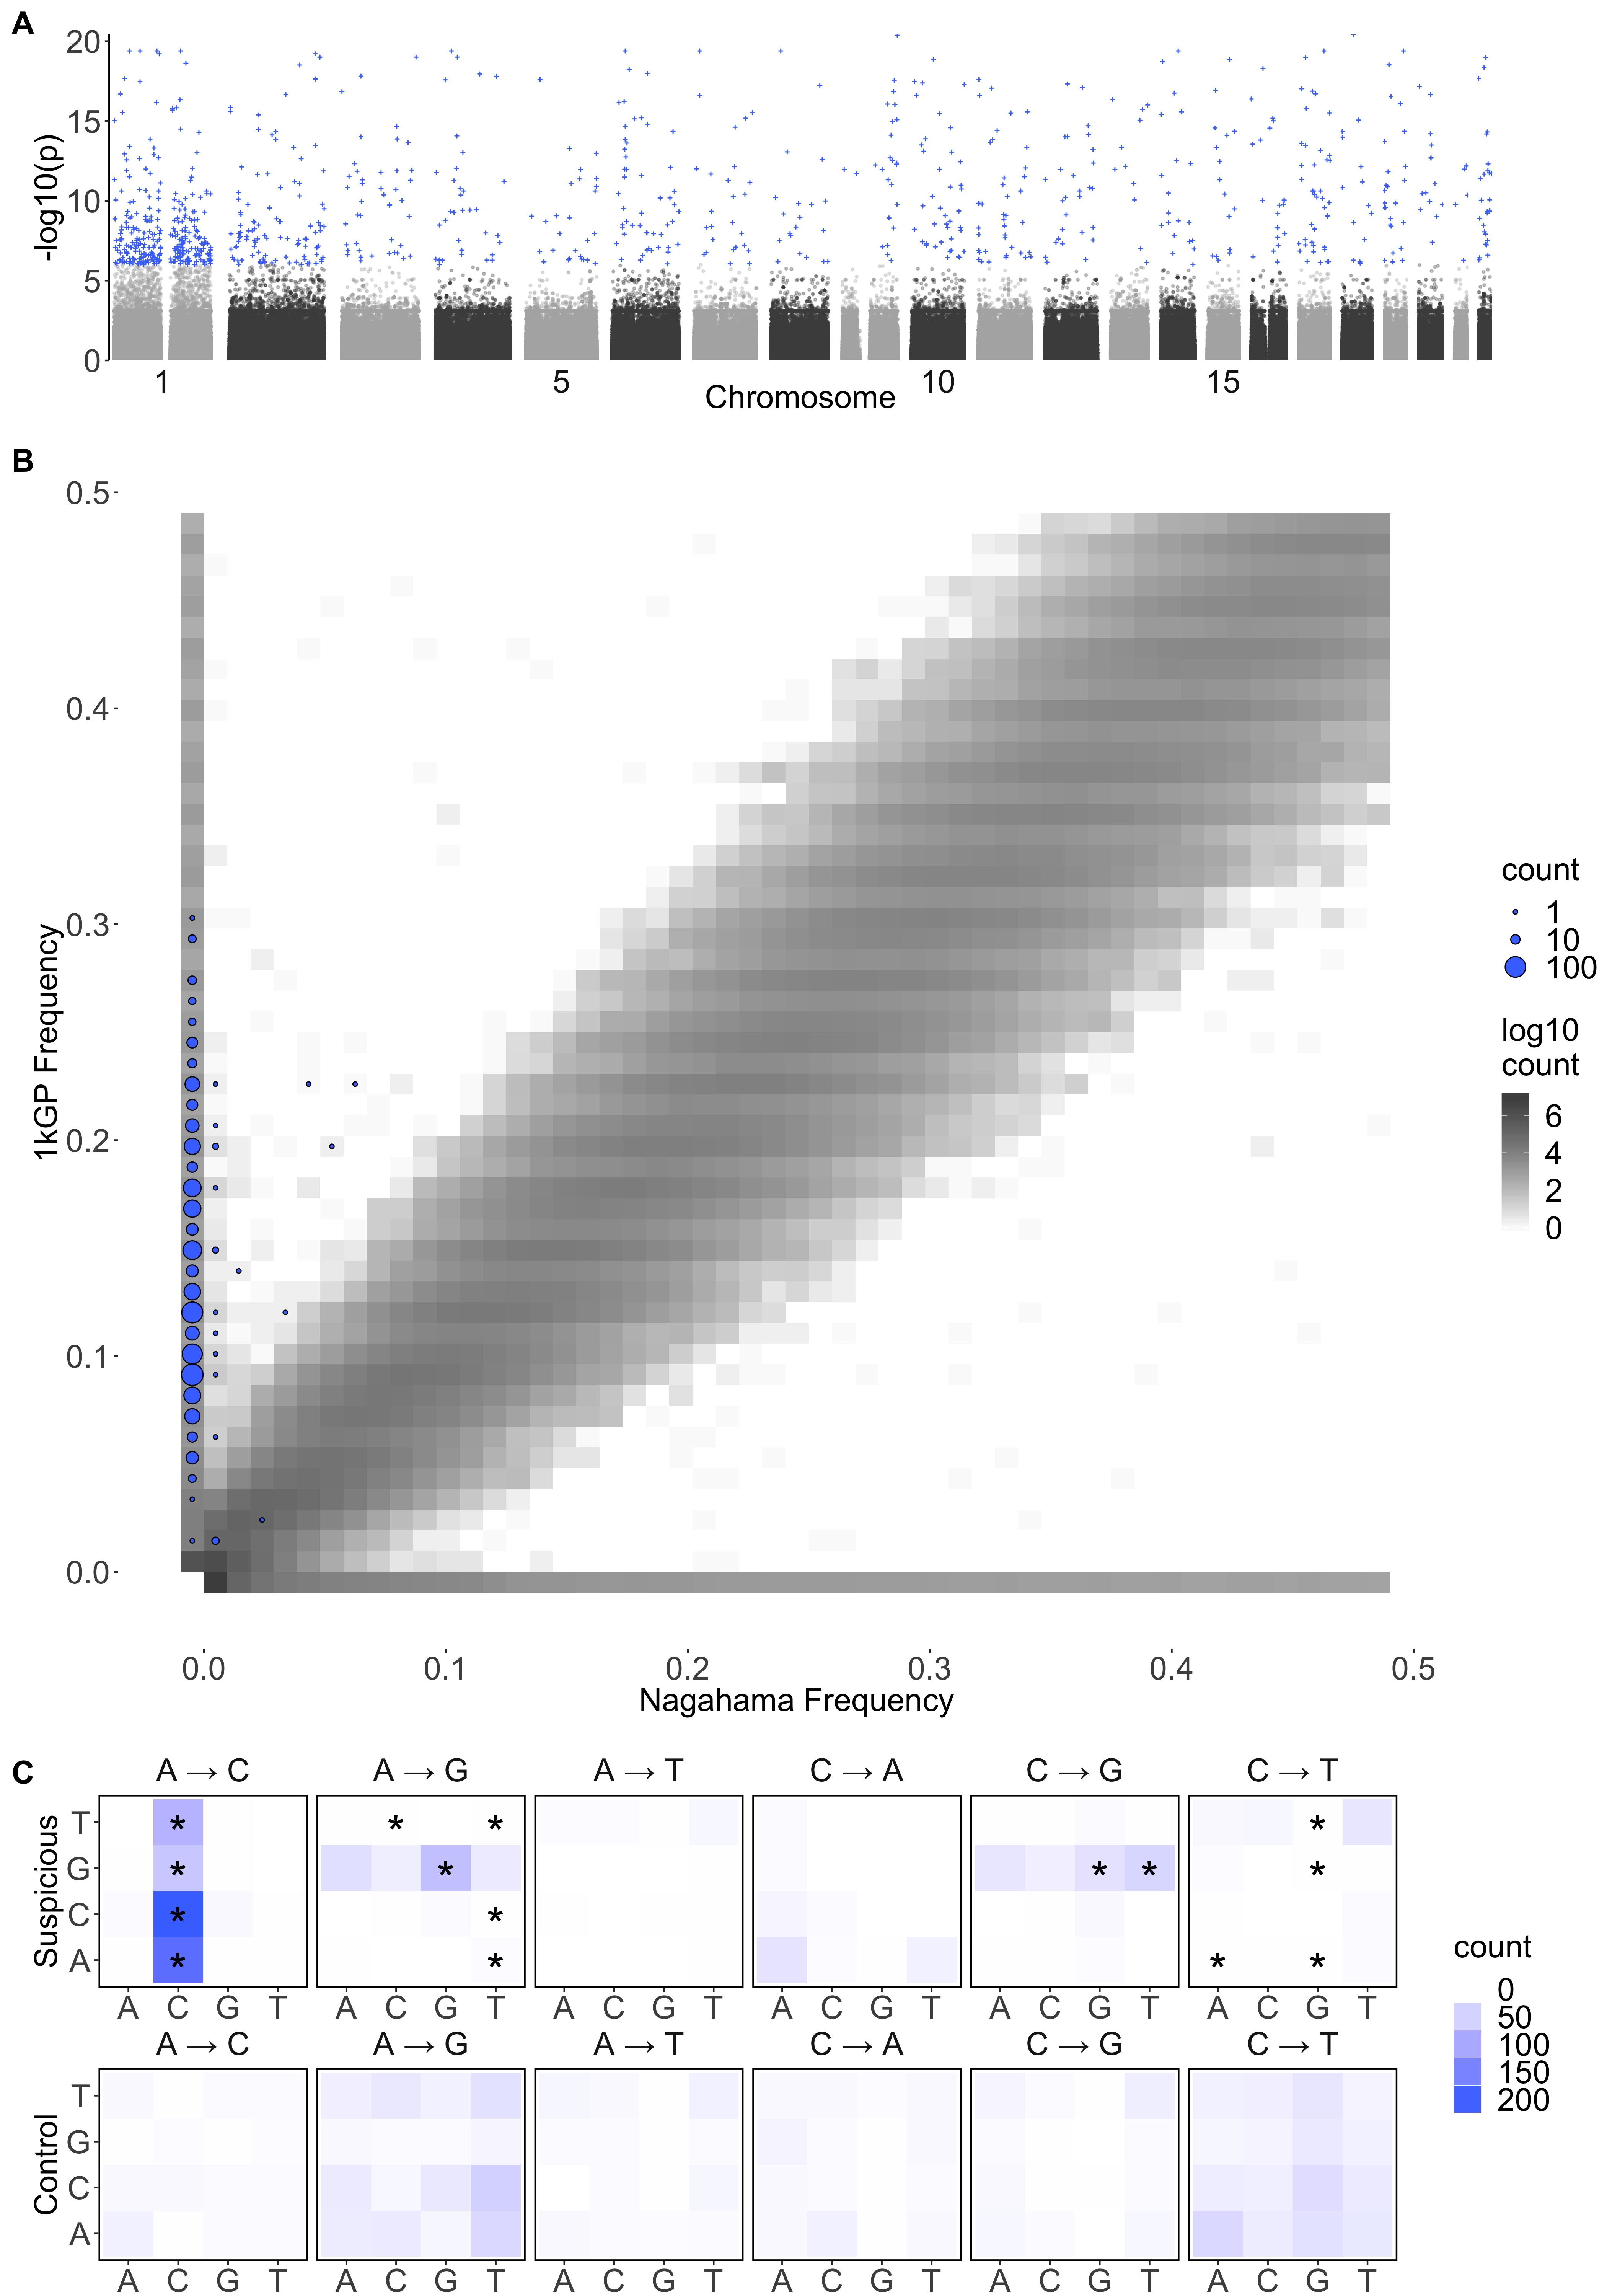
\includegraphics[width=\hsize,keepaspectratio]{./Figures/Figure1.jpg}
\caption{
\textbf{A} 
Mutation spectrum of the 1034 variants that reached a genome wide significance with a \textit{p}-value less than $p < 10^{-6}$  in a GWAS of sequencing quality. 
The majority of the variants with significant associations to $Q$ have the *AC${\rightarrow}$*CC mutational pattern. There is also a slight enrichment in GA*${\rightarrow}$GG* and GC*${\rightarrow}$GG* mutations. These three enrichments can be summarized as G**${\rightarrow}$GG*. (note: the reverse complement of *AC${\rightarrow}$*CC is GT*${\rightarrow}$GG*)
\textbf{B} 
Joint frequency spectrum plot of the Japanese from the 1kGP and a more recent Nagahama dataset.
Crosses ( + ) are variants that reached genome wide significance in a GWAS of sequencing quality. 
The histogram on the left of the plot is the distribution of significant variants. 
\textbf{C} 
Genome wide association of the average quality of mapped bases $Q$ for the 104 Japanese individuals included in the 1kGP. This GWAS identified $587\ \  p < 10^{-8}$ and $1034\ \ p < 10^{-6}$ SNPs that were associated to the average $Q$ of SNPs mapped for an individual
The same analysis was performed independently for each of the populations in the 1kGP. }
 \label{SFS}
\end{figure}

			\section{Results}
			
	\subsection{A peculiar mutational signature in Japan}			
	
Harris and Pritchard reported an excess of a 3-mer *AC${\rightarrow}$*CC mutational pattern in a portion of the Japanese individuals in the 1kGP \citep{Harris2015a}.
While trying to follow up on this observations in a larger and more recent Japanese cohort, we did not find this particular signature.
However, when comparing the allele frequencies between the Japanese individuals from the 1kGP and this larger dataset, we observed an unusually large number of single nucleotide polymorphisms (SNPs) private to one of the two groups.
This is unexpected given the similarity of the two populations, and suggests a technical difference rather than a population structure effect. 
Moreover, these mismatches were maintained after filtering for low-quality regions of the human genome and standard metrics such as Hardy-Weinberg equilibrium.
Low frequency variants have little power to detect Hardy-Weinberg disequilibrium, and in essence we would not expect any homozygous alternates for low frequency variants. 

When mismatch sites were removed from the 1kGP data, the  *AC${\rightarrow}$*CC signal disappears (Figure \ref{SFS}).
Regressions against different individual-level quality metrics provided by the 1kGP revealed that $Q$ per individual was an excellent correlate with prevalence of the  *AC${\rightarrow}$*CC mutational signature in 1kGP:
Individuals with low $Q$ show elevated rates of the signature (see Supplementary Figure \ref{PC1_Correlation}).
Thus, sequences with low quality harbour mutations that reproduce poorly across studies and exhibit a particular mutational signature. 

To identify SNPs that are likely to reproduce poorly across cohorts (without having access to a second cohort), we performed a \textit{reverse} genome wide association study (GWAS) in the JPT for SNPs that associate strongly with low $Q$ (Figure \ref{SFS}).
Traditionally, genome wide association studies use linear regression by predicting a phenotype based on genotype. 
In this case, we are using simple logistic regression looking for loci where the genotypes are predictable based on the data quality scores.
This approach identifies 587 SNPs with $p < 10^{-8}$ and 1034 SNPs with $ p < 10^{-6}$.
While identifying putative low-quality SNPs to exclude, using a higher $p$-value threshold increases the stringency of the filtering (i.e., excluding SNPs with $ p < 10^{-6}$ is more stringent than excluding SNPS with $p < 10^{-8}$). 
The variants that are associated to $Q$ have an enrichment in *AC${\rightarrow}$*CC mutations, GA*${\rightarrow}$GG*, and GC*${\rightarrow}$GG* mutations.
These three enrichments can be summarized as an excess of G**${\rightarrow}$GG* in individuals with low $Q$.

Thus, this mutational signal is heavily enriched in suspicious SNPs, but residual signal remains in non-significant SNPs, presumably because many rare alleles found in individuals with low $Q$ remain unidentifiable using association techniques. 
The removal of individuals with $Q$ below 30 successfully removes the *AC${\rightarrow}$*CC signal, however other signals identified by Harris and Pritchard appear unchanged. 
For population genetic analyses, the removal of individuals with low $Q$ appears preferable to filtering positions.

	\subsection{Identifying Suspicious SNPs in the 1kGP}
The results of the \textit{reverse} GWAS performed on the Japanese from the 1kGP lead us to consider whether any other populations in the 1kGP also had similar issues with data quality.
The $Q$ of individuals over time shows that the sequencing done in the early phases of the 1kGP was more variable and overall tended to include lower quality sequencing data (Figure \ref{MapQual}).
This variability could be as a result of fluctuating sequence platform protocols or variation between sequencing centres.
There were a number of protocols used to prepare the samples for sequencing, as well as a number of sequencing technologies used over the course of the data production.
By 2011, older sequencing technologies were phased out, and method development solidify, which coincides with the sequencing quality levelling off.
It is clear that there are many covariates that could be used to identify spurious sites such as sequencing date, sequencing technology or even the sequencing centre. 
However, the $Q$ per individual appeared to be the best metric to identify spurious sites.

The GWAS approach similarly identified $Q$-associated SNPs in 24 of the 26 populations in the 1kGP.
Over 3517 variants were independently associated to low $Q$ in at least two populations  (Figure \ref{OverLap}). We wanted a test statistic to represent the association across all populations; to do that we summed across the deviances from each population (adjusting the degrees of freedom for the chi-squared test according to the number of populations with a segregating variant) and identified 3990 statistically significant SNPs and 1134 statistically significant insertions and deletions (indels), as shown on Figure \ref{Manhattan} and Figure \ref{indel_Manhattan}.

\begin{figure}
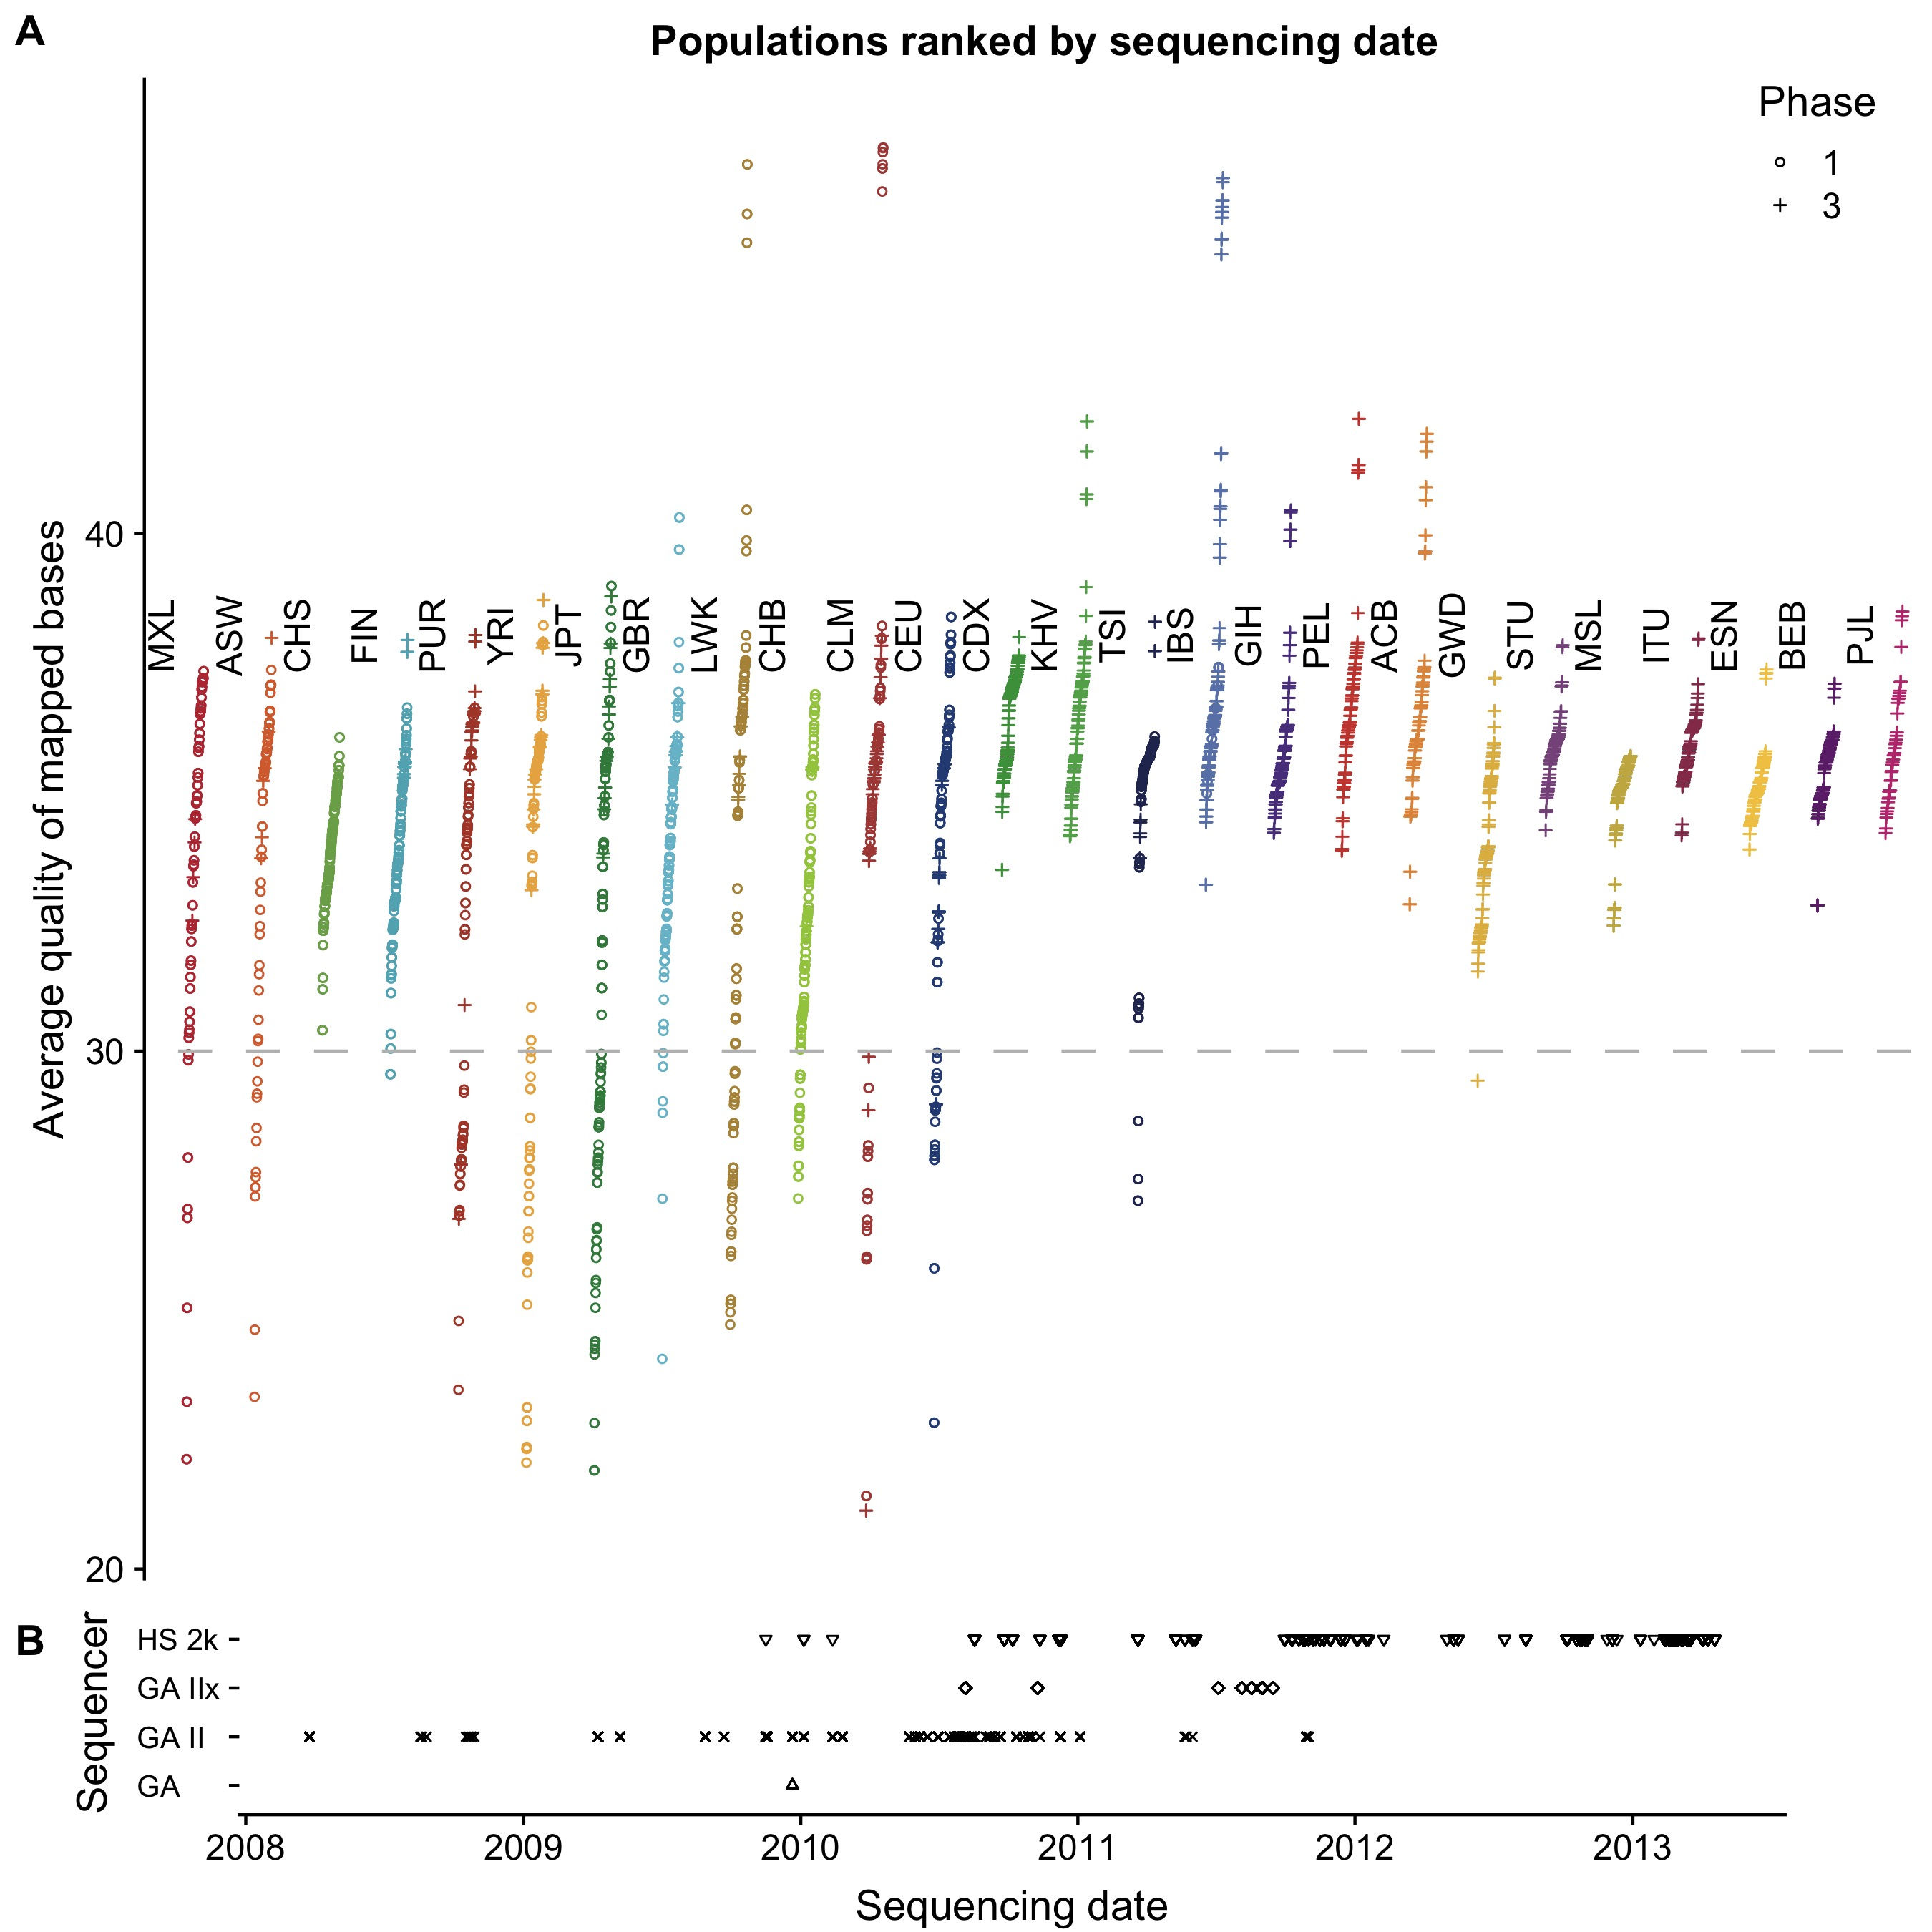
\includegraphics[width=0.95\hsize,keepaspectratio]{./Figures/MapQualOverTime.jpg}

\caption{\textbf{A}The average quality of mapped bases $Q$ for each individual per population included in the 1000 Genomes sequencing project. Individuals are ranked by the date of the earliest sequencing data is used for individuals sequenced more than once. The x-axis is ranked by the mean sequencing date per population. \textbf{B} The x-axis is sorted by the sequencing date per individual. The colours indicate the sequencing centres that produced the data for each individual and the shape indicates whether the individual belongs to Phase 1 or Phase 3 of the 1000 Genomes project. The bottom plot indicates the sequencing technologies used over time.}
\label{MapQual}
\end{figure}



\begin{figure*}
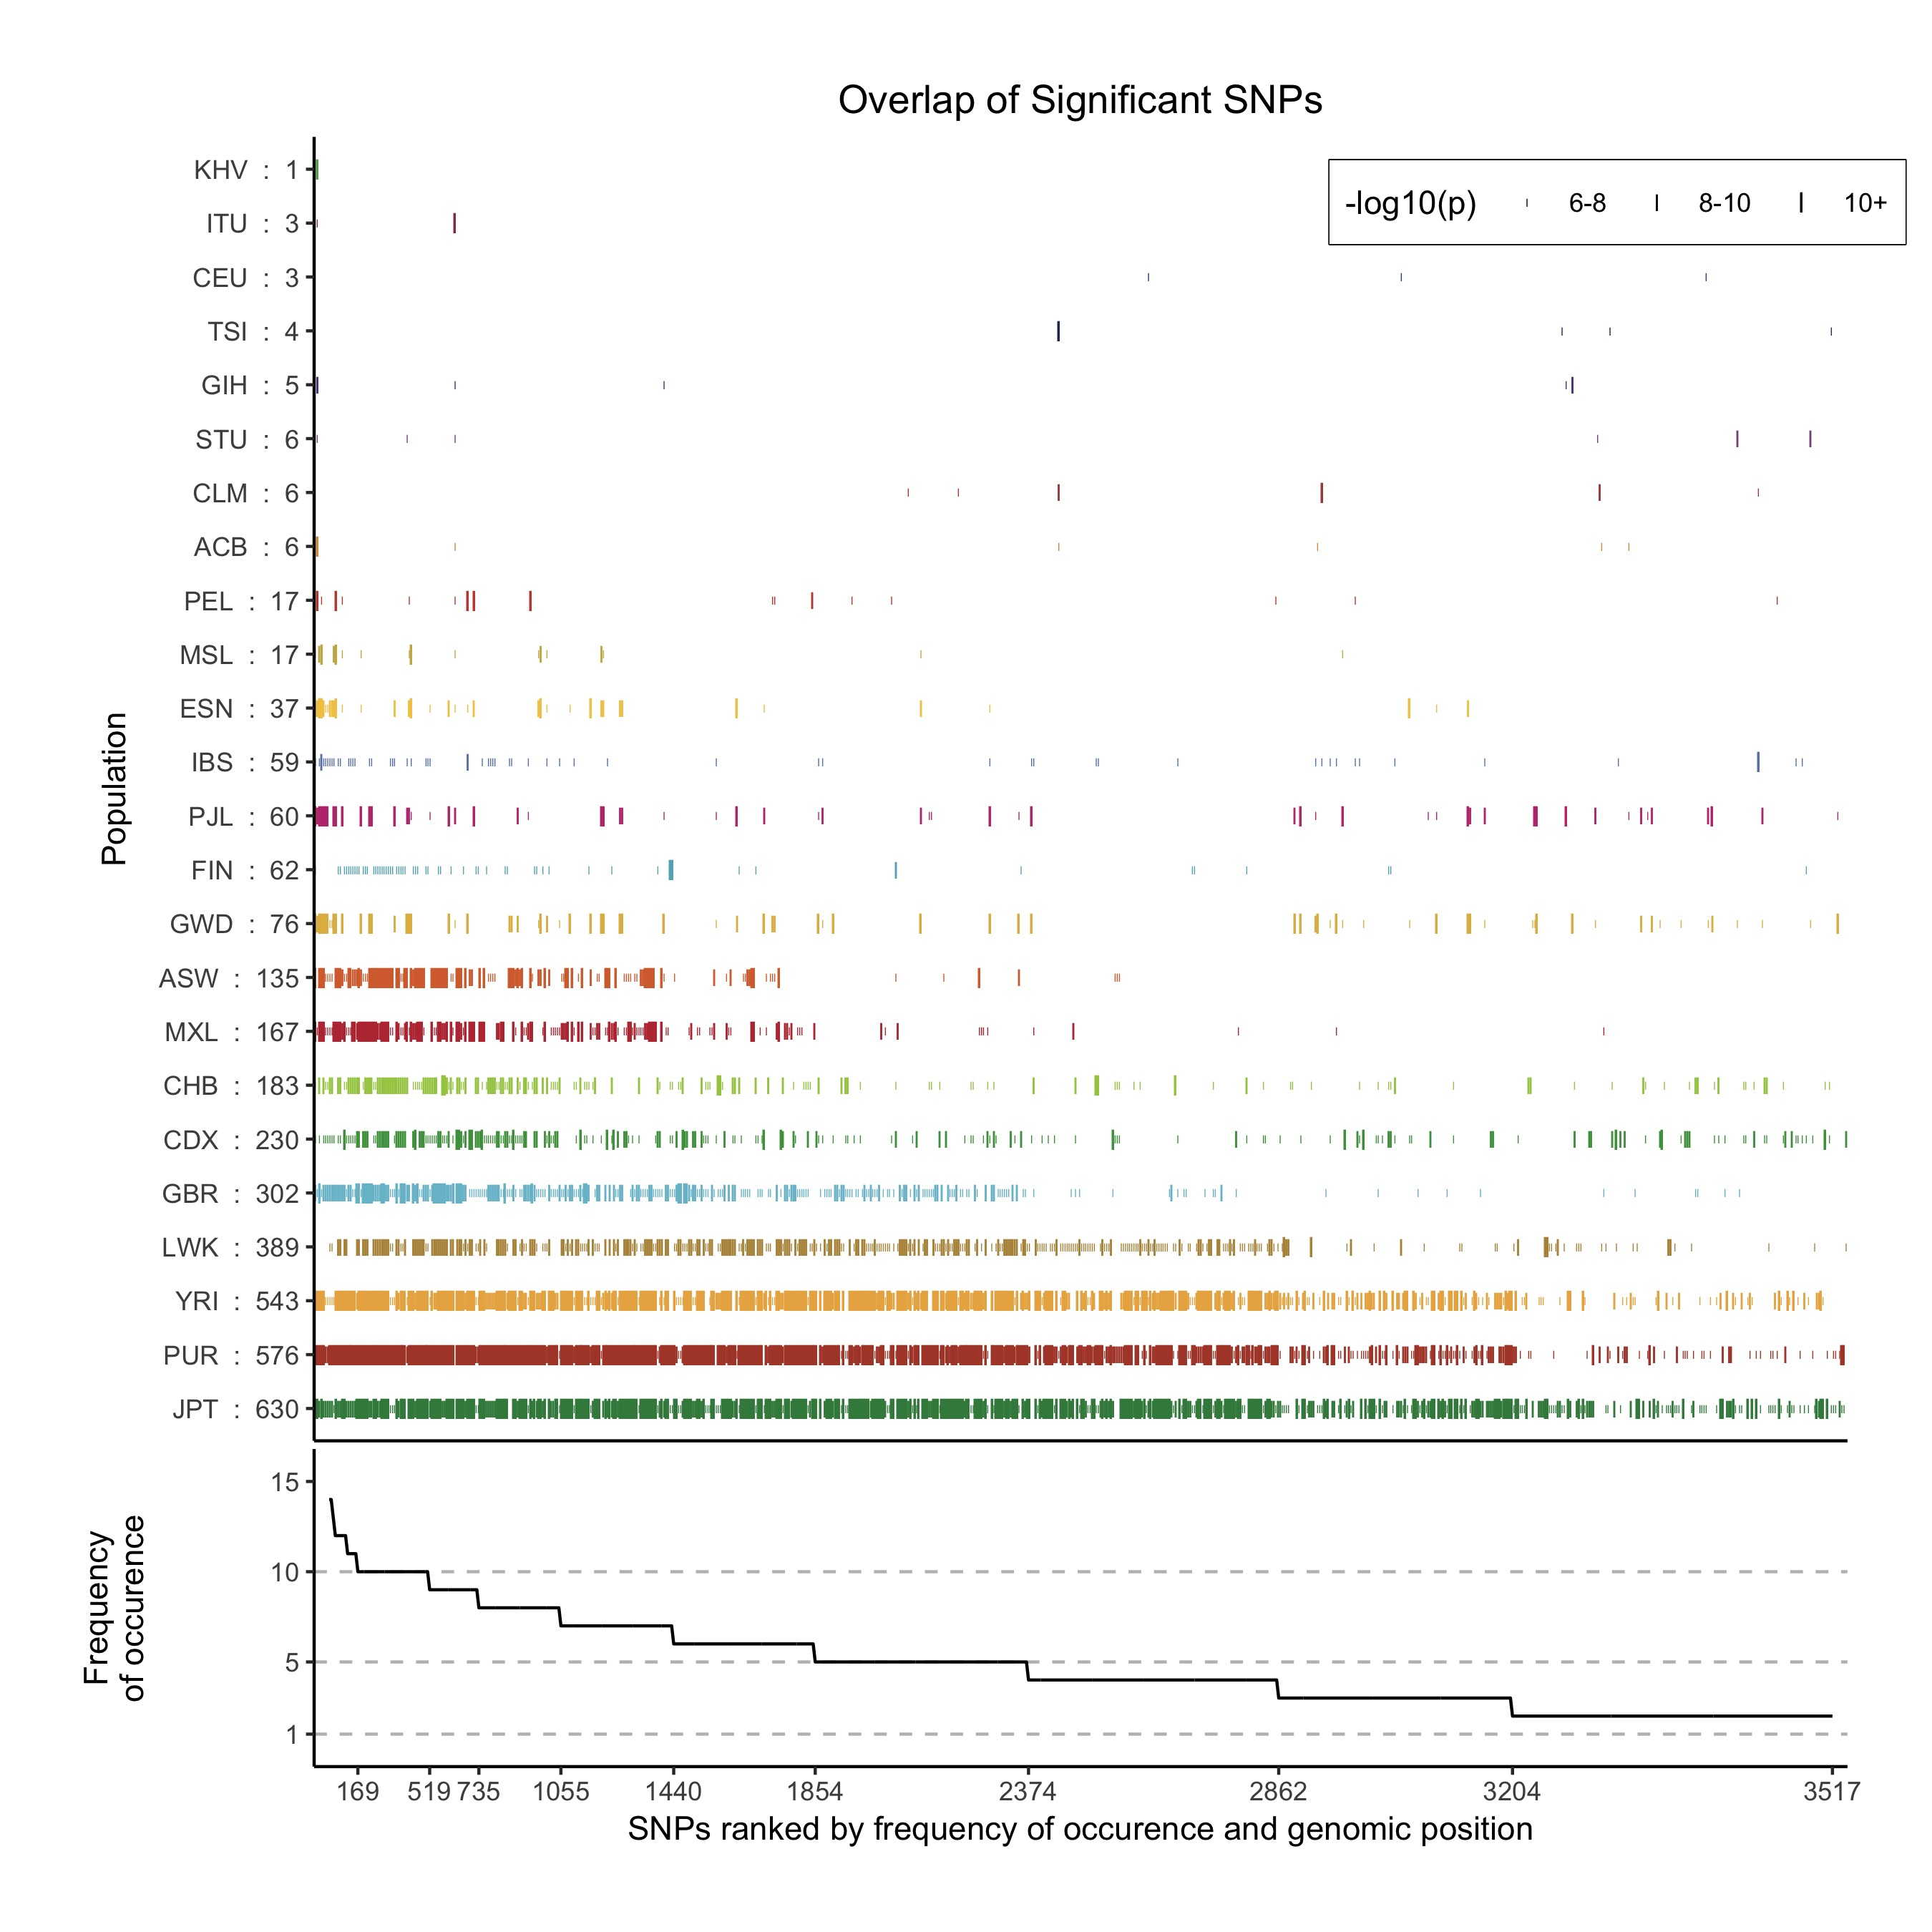
\includegraphics[width=\hsize,keepaspectratio]{./Figures/SNPOverlap6.jpg}

\caption{Overlap of SNPs identified independently to be associated with average quality of mapped bases $Q$. 
The size of the crosses ( + ) are proportional to the -log10(p) value of that SNP.
The x axis is ranked by the frequency of occurrence of a SNP, then by genomic position.
The line plot underneath shows the number of populations for which a variant has reached significance.
The populations that tend to have the most individuals with low $Q$ also tend to have the most variants associated to $Q$. 
The same variants identified as being low quality independently in each population are found in other populations. }
  \label{OverLap}
\end{figure*}

\subsection{Suspicious SNPs impact modern genomics analyses}
The state of the art imputation servers use a combination of many databases including many that are not freely available.
From the perspective of researchers, they act as black-box imputation machines that take observed genotypes as input and return imputed genotypes.  
In order to investigate the proportion of variants that we have identified as being associated to $Q$ that are being imputed, we submitted genotype data from all of the 1kGP individuals to the Michigan Imputation Server.
We found that all of the SNPs we identified as being associated with $Q$ for chromosomes 1 and 2 were imputed. 
This suggests that the imputation reference panel likely includes individuals with low $Q$, and the dubious variants have not been removed. 


Once we identified SNPs that were clearly associated with low $Q$, we searched the literature for any GWAS that might have reported these dubious variants as being significantly associated with some biological trait. 
The NHGRI-EBI Catalog of published genome-wide association studies identified two recent publications that had found variants to have either reached or nearly reached genome wide significance of $ p < 10^{-8}$.

One of these studies genotyped individuals and imputed the data using the HapMap II as a reference  database for imputation.
The other study used the 1kGP sequence data and cell lines directly.
Both papers used strict quality thresholds, including population genetic statistical tests such as the Hardy-Weinberg equilibrium test, deviations in expected allele frequency and sequencing data quality thresholds. 
They also removed rare alleles and alleles with high degrees of missingness. 
Despite using state-of-the-art quality controls, these erroneous variants managed not only to be imputed onto real genotype data, but they also reached genome wide significance for biological traits.

\section{Discussion}
One paper identified SNPs associated to ADHD using a GWAS on quantitative measures of ADHD symptoms.
While none of their SNPs reached significance below $ p < 10^{-8}$, they reported their results below a significance threshold of $ p < 10^{-5}$.
The data used was imputed genotype data using Hapmap II as the reference.
One of the top 25 SNPs in the GWAS on ADHD (rs6057648) was identified as being significantly associated to $Q$ \citep{Ebejer2013}.
While they are clear in reporting that these SNPs are not genome wide significant, one can imagine a meta-analysis using this dataset would include the false positive SNP we identified.
Finding some of these SNPs in HapMap data was unexpected, however, not impossible considering that HapMap and 1kGP shared many samples.
We found that roughly 1\% of the SNPs associated to $Q$ were found in HapMap; rs6057648 is among those found in HapMap.

Another paper used the raw BAM files from the 1kGP to identify EBV copy number by comparing the number of reads that mapped to EBV.
They did PCR confirmation of EBV copy number using 7 samples from some of the populations, although as it turns out, all of these samples have relatively high $Q$.
They performed a GWAS on the EBV copy number and identified only one SNP with significance below $ p < 10^{-8}$. 
They also reported the SNPs reading significance below $ p < 10^{-6}$. 
Four of the SNPs in the top hits of the Asian populations (rs200655768, rs184202621, rs201255786, rs201761909) were identified by our regression against $Q$ \citep{Mandage2017}.

The EBV strain was used to transform B-cells from blood samples from the 1kGP into lymphoblastoid cell lines.
This is a commonly used transformation that helps preserve cell lines for long periods of time.
It is unclear what exactly might be causing the association to EBV copy number and the data quality, however, one could speculate that different protocols were used in the cell culturing of certain samples from the 1kGP which might affect the replication of the virus in the cells, or somehow affect the overall quality of the sequencing data produced.
Further investigations in the source of the issue could be done using the raw sequence data from the 1kGP along with the per sample per base quality metrics. 			

\subsection{Technical Artifact}
The variants identified in this study are likely to be technical artifacts from legacy technology.
Different sequencing technologies will have different error profiles. 
A report comparing the Genome Analyzer II (GAII) to the Illumina HiSeq found that the GAII had much higher rates of reads below a quality score of 30 \citep{Minoche2011}, with, for instance, different patterns of quality decrease along reads (known as B-tails). 
Differences in read quality and error profiles in turn require different calling pipelines.

We were not able to pinpoint the precise technical source of the discrepancy. Sequencer-specific errors would be expected to be absent from Hapmap, which was sequenced with an entirely different platform. \sgcomment{Check that is sanger, if so, say so}. We find that \sgcomment{$99\%$--check} of the suspicious snps are indeed absent from HapMap, which is consistent with the expected false positive rate in our test.   
  
The presence of some of these SNPs in HapMap suggests a cell line effect; although, this result is not very convincing with only 1\% of sites identified in 1kGP present in HapMap.
Indeed, further inquiries into the details of sample preparation and data processing would be required to identify the source of this signal. 

If these sequencing platforms are no longer being used, then it it likely that these artifacts are no longer being actively introduced in recent sequence data.
However, because the 1kGP data is widely used as a reference database, these variants are being imputed onto new genotype data.
We have shown that these variants have been significantly associated using traditional GWAS methods.
However, this is not the only method that would be affected by these false positives. 
Polygenic risk scores, meta analyses and other methods that combine the scores of multiple variants might also include some of these variants in their analyses.
The inclusion of these variants could also affect population genetics analyses that compare and contrast populations based on allele frequencies.


\subsection{Recommendations}
While it may be difficult to determine the exact source of the bias in the data, we have been able to identify individuals and loci that do not meet the current quality standards.
A conservative approach would be to remove all individuals that do not meet the quality threshold as well as all the variants associated to low $Q$.
In this case, we used a cut-off of $Q$ over 30.
Another approach is to remove all the sites that reach a significance below $ p < 10^{-6}$ in at least two populations or using the sites reaching a significance below $ p < 10^{-6}$ in the combined test. (See supplementary material for lists of SNPs)

\section{Conclusion}

On a technical front, we were surprised that strong association between SNPs and technical covariates in the 1kGP project had not been identified before. 
The genome wide simple logistic regression analysis approach is rather straightforward, and could be a standard in a variety of -omics studies. 

More generally, to improve the quality of genomic reference datasets, we can proceed by addition of new and better data and by better curation of existing data.
Given rapid technological progress, the focus of genomic research is naturally on the data generation side. However, cleaning up data is also important to avoid generating spurious results. 
The present findings suggest that a substantial fraction of the final release of the 1kGP project is overdue for removal or re-sequencing. 

We have not identified the precise mechanism through which the technical artifact was introduced: we have ruled out neither cell-line, sequencer, nor algorithmic artifact. 
Given that modern platforms seem to have resolved this technical issue but that recent studies continue to be affected by the legacy batch effect, we found it worthwhile to draw attention to the statistical artefact while the sequencing forensics investigation can take place.     


\section{Methods}
\subsection{Metadata}
The metadata used in this analysis was compiled from each of the index files from the 1000 Genomes file system. 
Average quality of mapped bases $Q$ per sample was obtained from the BAS files associated with each alignment file. 
Each BAS file has metadata regarding each sequencing event for each sample. 
If a sample was sequenced more than once, we took the average of the each $Q$ score from each sequencing instance. 
The submission dates and sequencing centres for each sample in the analysis was available in the sequence index files.  
This file also has multiple entries per sample, however, we were unable to match the individual sequencing runs between the bas files and the index file, which lead us to take the average of the $Q$ scores and only kept the earliest sequencing date per sample. 
The dates of the sequencing are only used to plot Figure.

\subsection{Data Availability}

Index of BAS files \href{http://ftp.1000genomes.ebi.ac.uk/vol1/ftp/data_collections/1000_genomes_project/1000genomes.low_coverage.GRCh38DH.alignment.index}{available here}.

Phase3 analysis sequence index file  \href{http://ftp.1000genomes.ebi.ac.uk/vol1/ftp/phase3/20130502.phase3.analysis.sequence.index}{available here} 

\todo{link to my compiled metadata file here}

\subsection{Quality Controls}
We reproduced the quality control pipelines used by Harris et. al as they applied the current state of the art quality thresholds to remove questionable sequences especially for the high standards for detecting population level differences. 
Several mask files were applied to remove regions of the genome that might be lower quality, or might have very different mutation rates or base pair complexity compared to the rest of the genome. 
The  1000 Genomes \href{http://ftp.1000genomes.ebi.ac.uk/vol1/ftp/release/20130502/supporting/accessible_genome_masks/20141020.strict_mask.whole_genome.bed}{strict mask} was used to remove low quality regions of the genome , highly conserved regions were removed using the \href{http://hgdownload.cse.ucsc.edu/goldenPath/hg19/database/phastConsElements100way.txt.gz}{phastCons100way} mask file and highly repetitive regions were also removed using the \href{http://hgdownload.cse.ucsc.edu/goldenpath/hg19/database/nestedRepeats.txt.gz}{NestedRepeats} mask file from RepeatMasker. 
Furthermore, only sites with missingness below 0.01, MAF less than 0.1, and MAF greater than 0.9 we're considered.
In total, 57,838,849 diallelic autosomal SNPs passed our quality controls for the mutation spectrum analysis and reverse GWAS. 
We also ran the same reverse GWAS separately on 2,952,684 insertions and deletions that passed the same quality controls.

\subsection{Genome wide association study}
We ran a simple logistic regression independently for each combination of genomic locus $s$ and population $p$ using the R glm package\citep{RDevelopmentCoreTeam2016}. The model we fitted to each subset of data can be expressed as such.
\begin{align*}
{logit}{E(Y_{s'p'i})} &= \beta_{0}^{(sp)} + \beta_{1}^{(sp)} Q_{p'i}
\\
\textit{for}\quad i &= 1,\hdots, n_{p'}
\end{align*}
Here $Y_{spi}$ is a Bernoulli random variable denoting the genotype of individual $i$ in population $p$ at genomic locus $s$. 
In the model, the regression coefficient $\beta_{0}^{(sp)}$ represents the baseline allele frequency in population $p$, the slope coefficient $\beta_{1}^{(sp)}$ denotes the association to average quality of mapped bases $Q_{p}$ to genotype $Y_{sp}$. 
We run a total of $K (= \sum_{s=1}^S P_s)$ regressions, where $S$ is the total number of genomic loci, and $P_s$ is the number of populations with a segregating variant for locus $s$. 
In the data, $P_s$ ranges from 1 to 26 since not all SNPs were present in all populations with singletons and doubletons filtered out.

For each of the $K$ regressions, we formulated a null hypothesis $H_{0}: \beta_{1}^{(sp)}=0$. That is, the average quality of mapped bases $Q_{p}$ variable is not associated with genotype $Y_{sp}$.
In other words, the slope coefficient of the simple logistic regression is zero.
To test the null hypothesis, we used the chi-square likelihood ratio test statistic (the deviance) as a measure of the marginal importance of adding $Q_{p}$ in the model. 
The deviance test statistic is approximately chi-square distributed with one degrees of freedom.  

To obtain a population-wide measure of association for each locus across its respective $P_s$ populations, we summed the $P_s$ deviances for each $s$. The resulting test statistic $T_s$ is chi-squared distributed with $P_s$ degrees of freedom (i.e. $T_s \sim \chi^2_{P_s}$), see Figure \ref{Deviances}.
The observed summed deviances were used to compute the \textit{p}-value for each locus.


Given the large number of tests (of which there are $S$), the large proportion of expected null hypotheses and the positive dependencies across the genome, we used the two-stage Benjamini \& Hochberg step-up FDR-controlling procedure to adjust the \textit{p}-values \citep{Benjamini2006}.
By using a nominal Type-I error rate $\alpha = 0.01$, a total of 3990 SNPs and 1134 indels were found to be statistically significance. See supplementary file {here}. \luke{make this file}

\subsection{Mutation Spectrum}
We calculated the mutation spectrum of triplets for the list of significant SNPs for the JPT population using a similar method as described in Harris et al. 2017. \citep{Harris2017a}
We modified the methods as necessary for our purposes, scripts are available \href{https://github.com/LukeAndersonTrocme/QualityPaper}{here}. 

\subsection{Imputation}
Using the Michigan Imputation Server, we imputed the genotype data from 1kGP for chromosomes 1 and 2.
We used the genotyped data from the 1kGP \href{ftp://ftp.1000genomes.ebi.ac.uk/vol1/ftp/release/20130502/supporting/hd_genotype_chip/ALL.chip.omni_broad_sanger_combined.20140818.snps.genotypes.vcf.gz}{Omni chip} genotype data.
The VCF file returned from the server was then downloaded and used to search for the number of significant SNPs successfully imputed.

\section{Code Availability}
https://github.com/LukeAndersonTrocme/QualityPaper

\section{Acknowledgments}
We would like to thank Kelly Harris for sharing her mutation spectrum scripts.

\bibliography{Legacy.bib}

\clearpage
\section{Supplementary Figures}

\renewcommand{\thefigure}{S\arabic{figure}}
\setcounter{figure}{0}   	

\begin{figure}
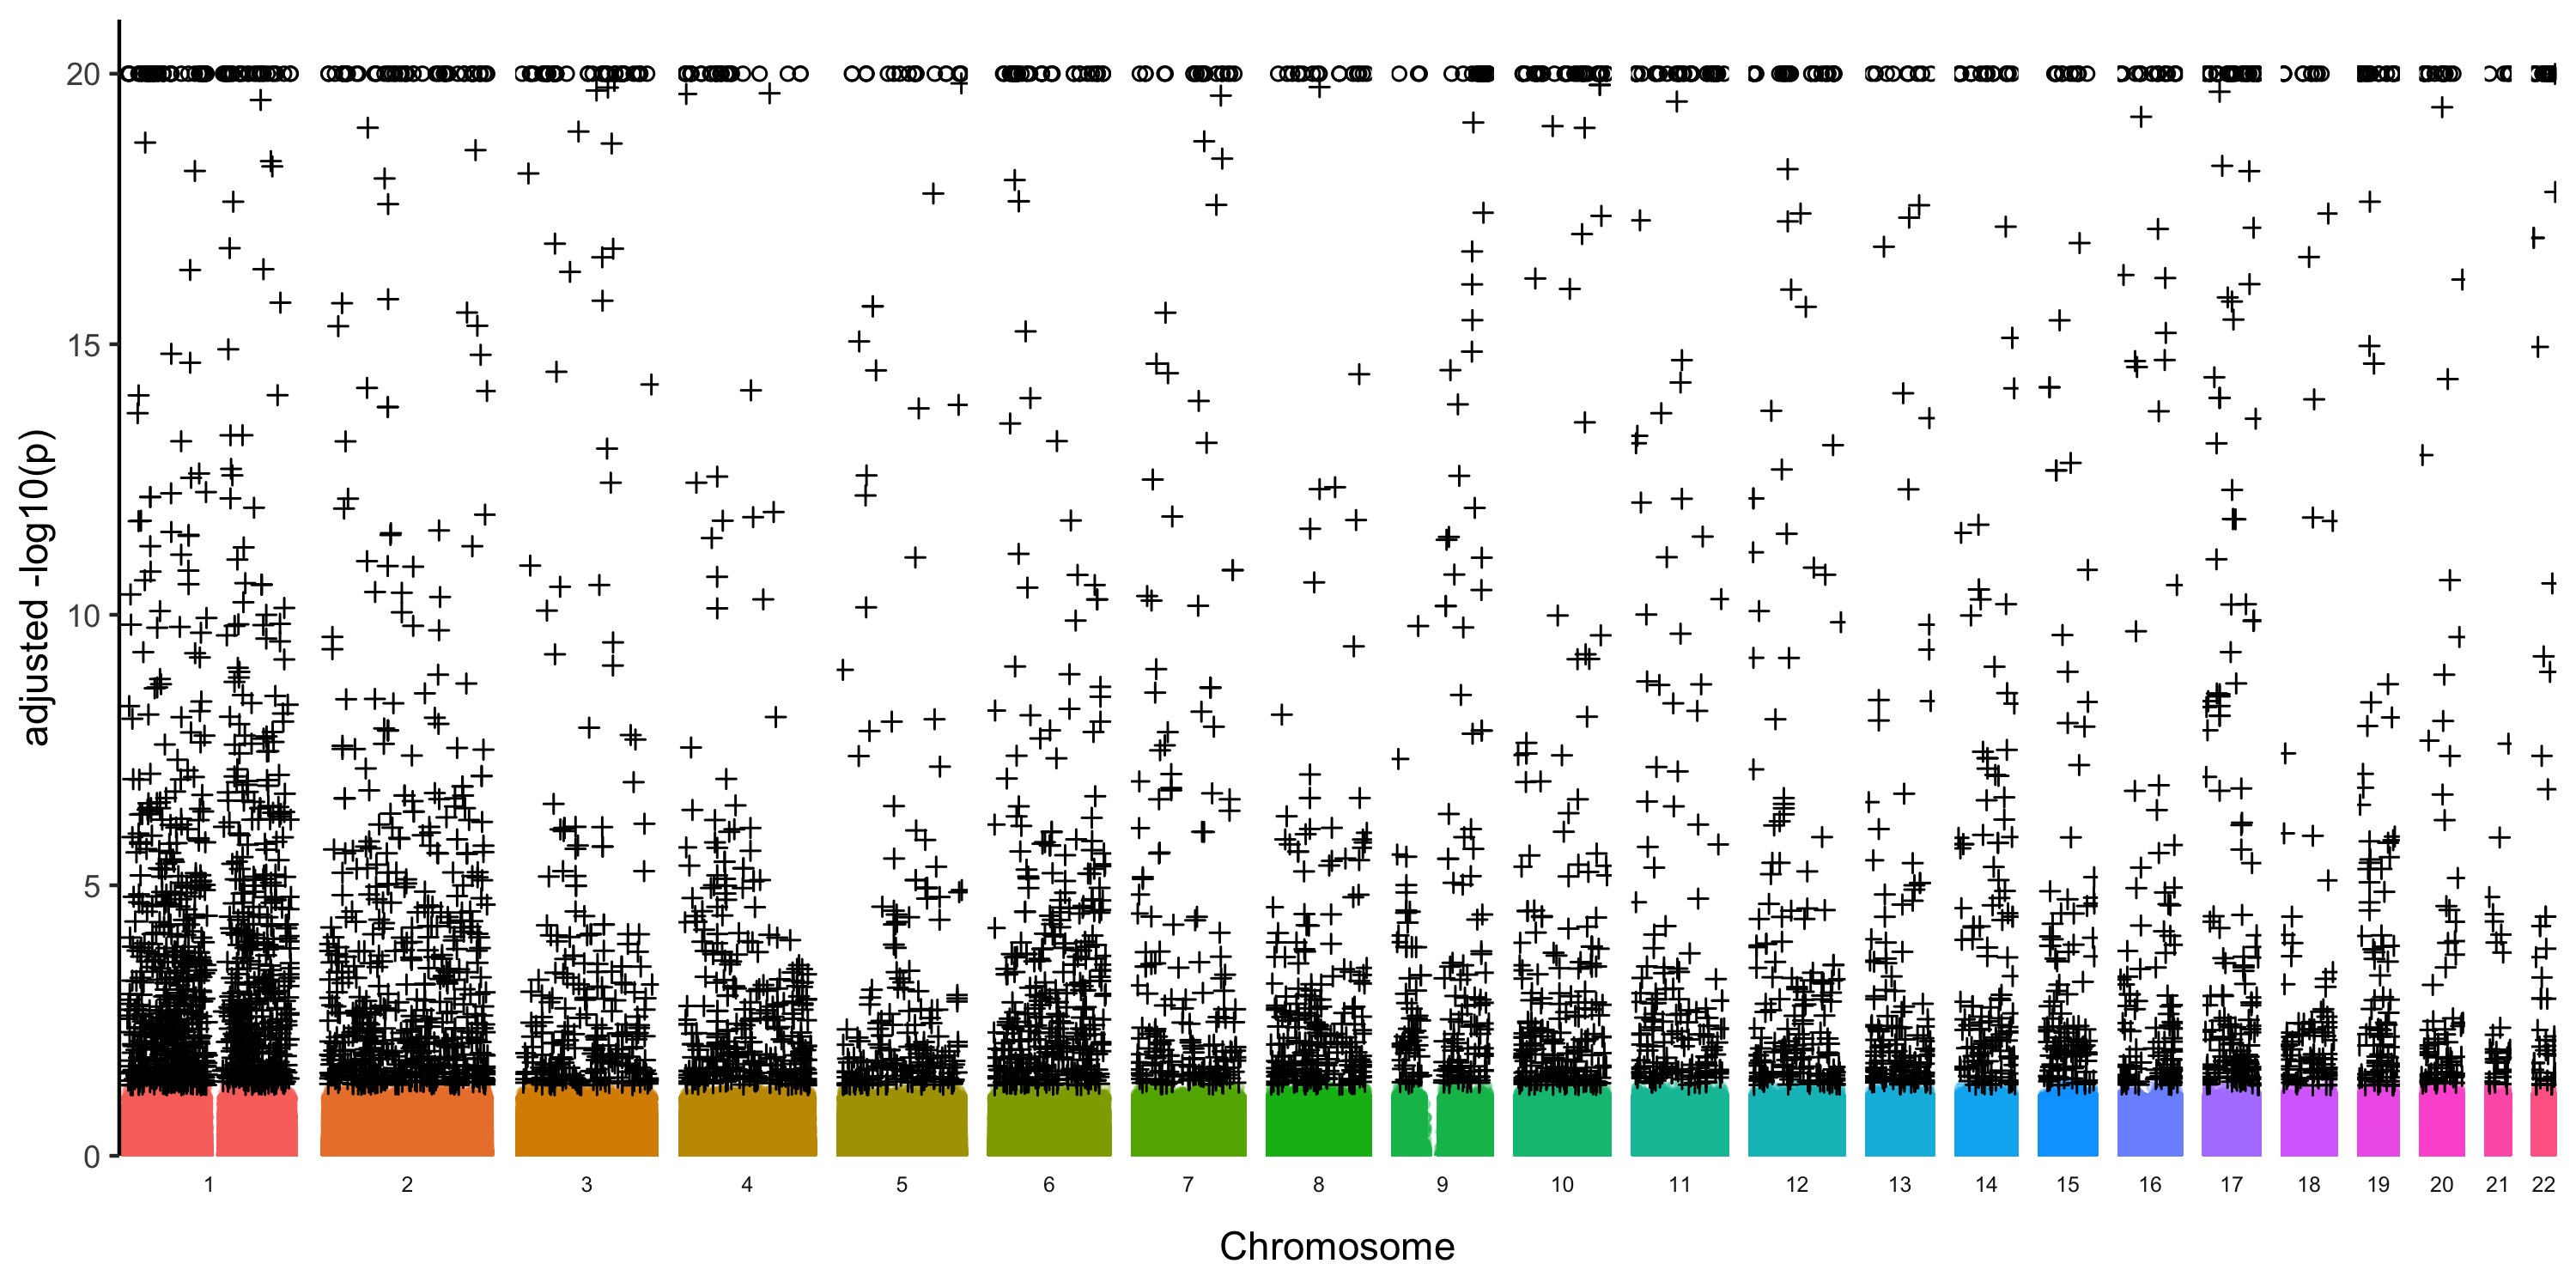
\includegraphics[width=\hsize,keepaspectratio]{./Figures/ManhattanPlot_adjusted.jpg}

\caption{Manhattan plot of the -log10 p values for the combined test using the deviances from each population of the 1kGP. 
There are 3990 variants that reach p values greater than $ p < 0.01$ after performing a two-stage Benjamini and Hochberg FDR adjustment. 
The circles ( o ) are SNPs that reached values greater than 20, for clarity we implemented hard ceiling at 20.}
  \label{Manhattan}
\end{figure}

\begin{figure}
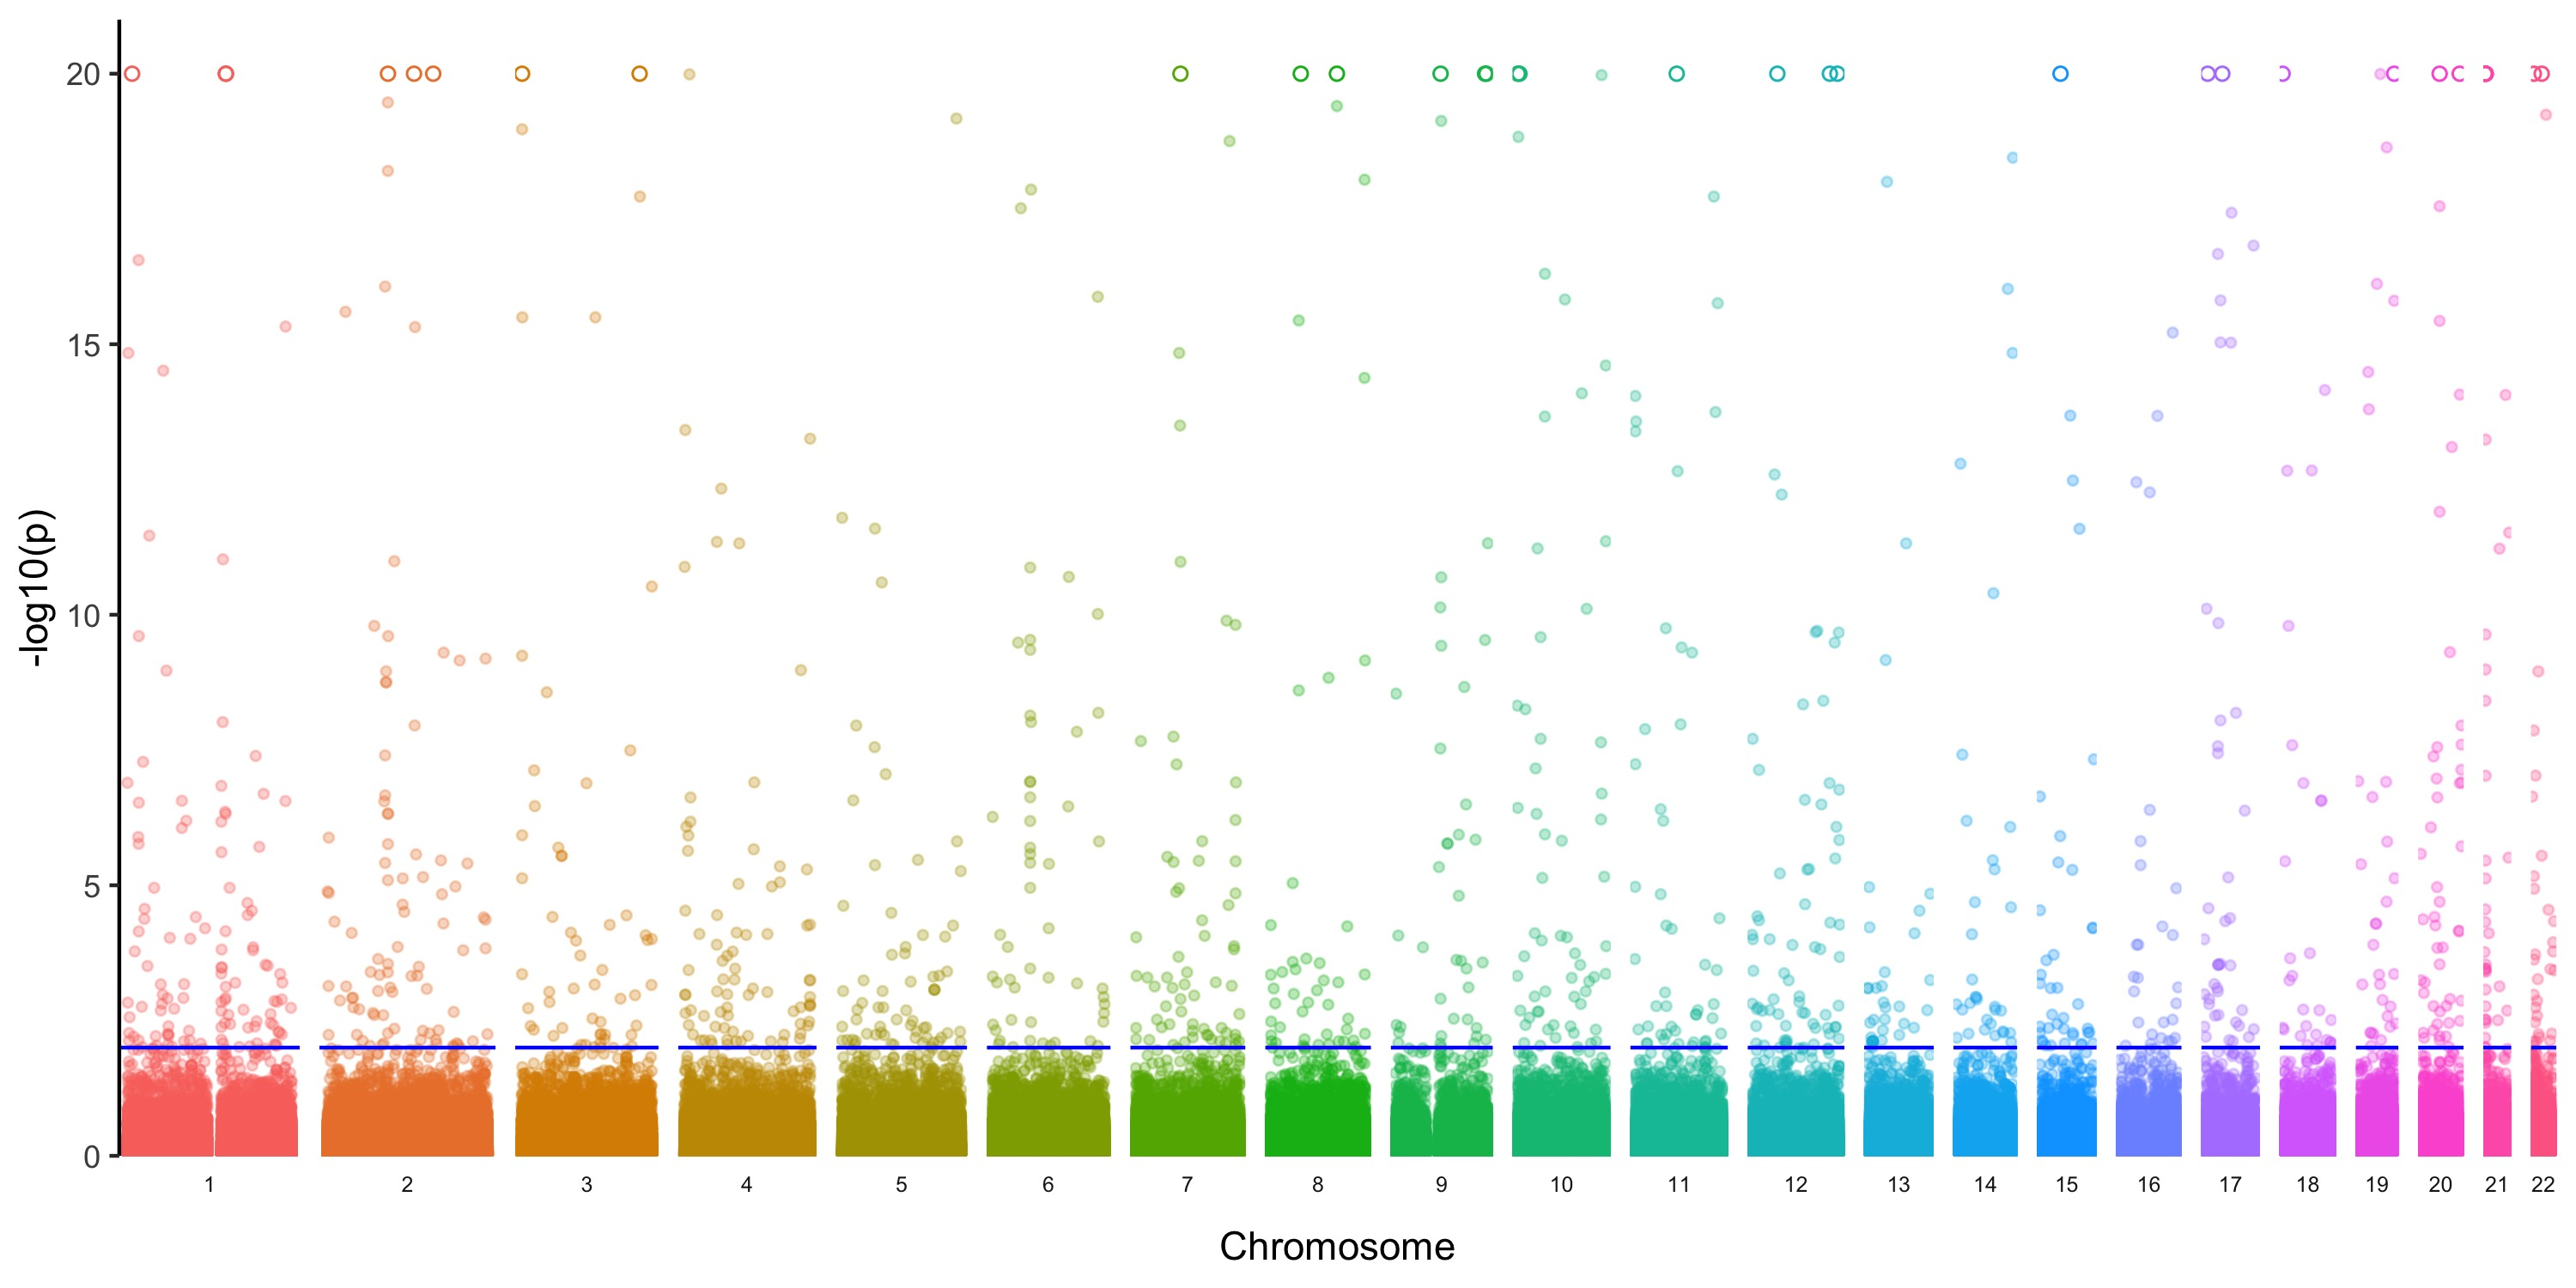
\includegraphics[width=\hsize,keepaspectratio]{./Figures/ManhattanPlot_indels.jpg}

\caption{Manhattan plot of the -log10 p values for the combined test using the deviances from each population of the 1kGP. 
There are 1134 insertions and deletions that reach p values greater than $ p < 0.01$ after performing a two-stage Benjamini and Hochberg FDR adjustment. 
The circles ( o ) are SNPs that reached values greater than 20, for clarity we implemented hard ceiling at 20.}
  \label{indels_Manhattan}
\end{figure}

\begin{figure}
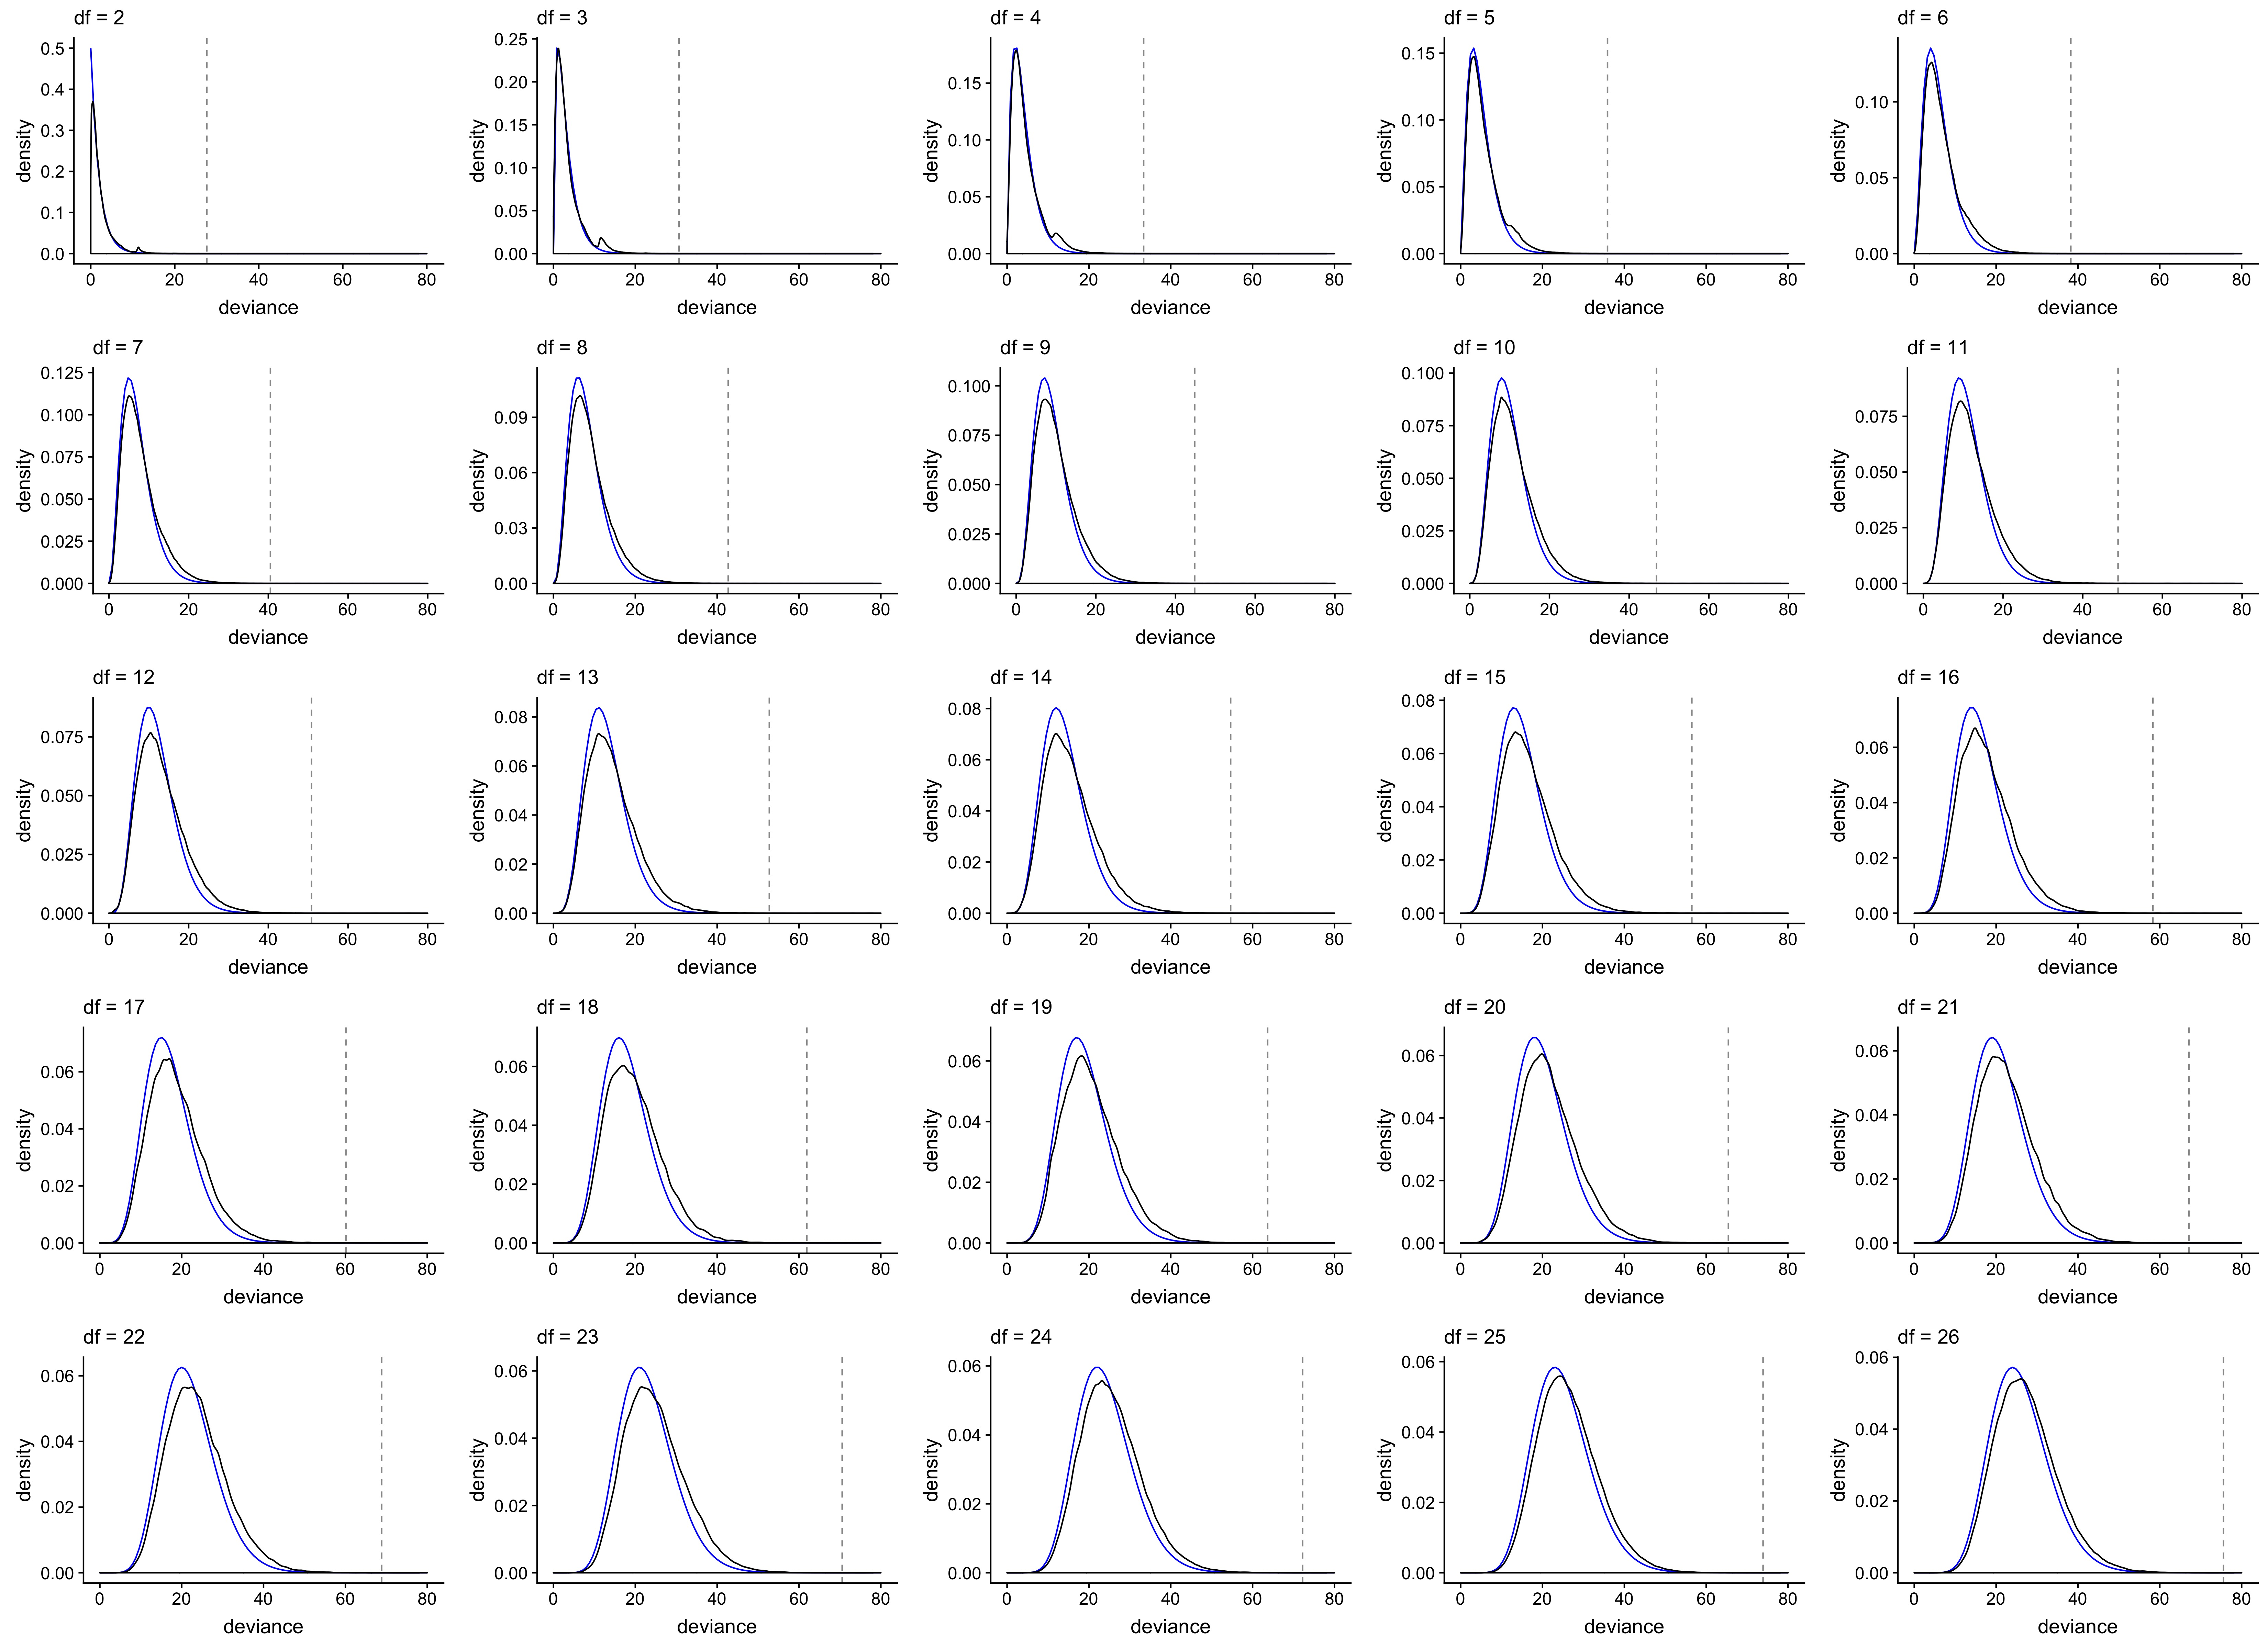
\includegraphics[width=\hsize,keepaspectratio]{./Figures/AllDeviances.jpg}

\caption{Empirical distribution plots of the sum of deviances grouped by N, the number of populations included. The blue curve is the theoretical null reference chi squared distribution with $N$ degrees of freedom. Note $\sum_i^N  \chi^2_1= \chi^2_N$. The grey dotted line indicates the significance level of $10^{-5}$ for the respective distribution which happens to be very close to the adjusted \textit{p}-value threshold at 0.01 FDR. }
\label{Deviances}
\end{figure}

\begin{figure}
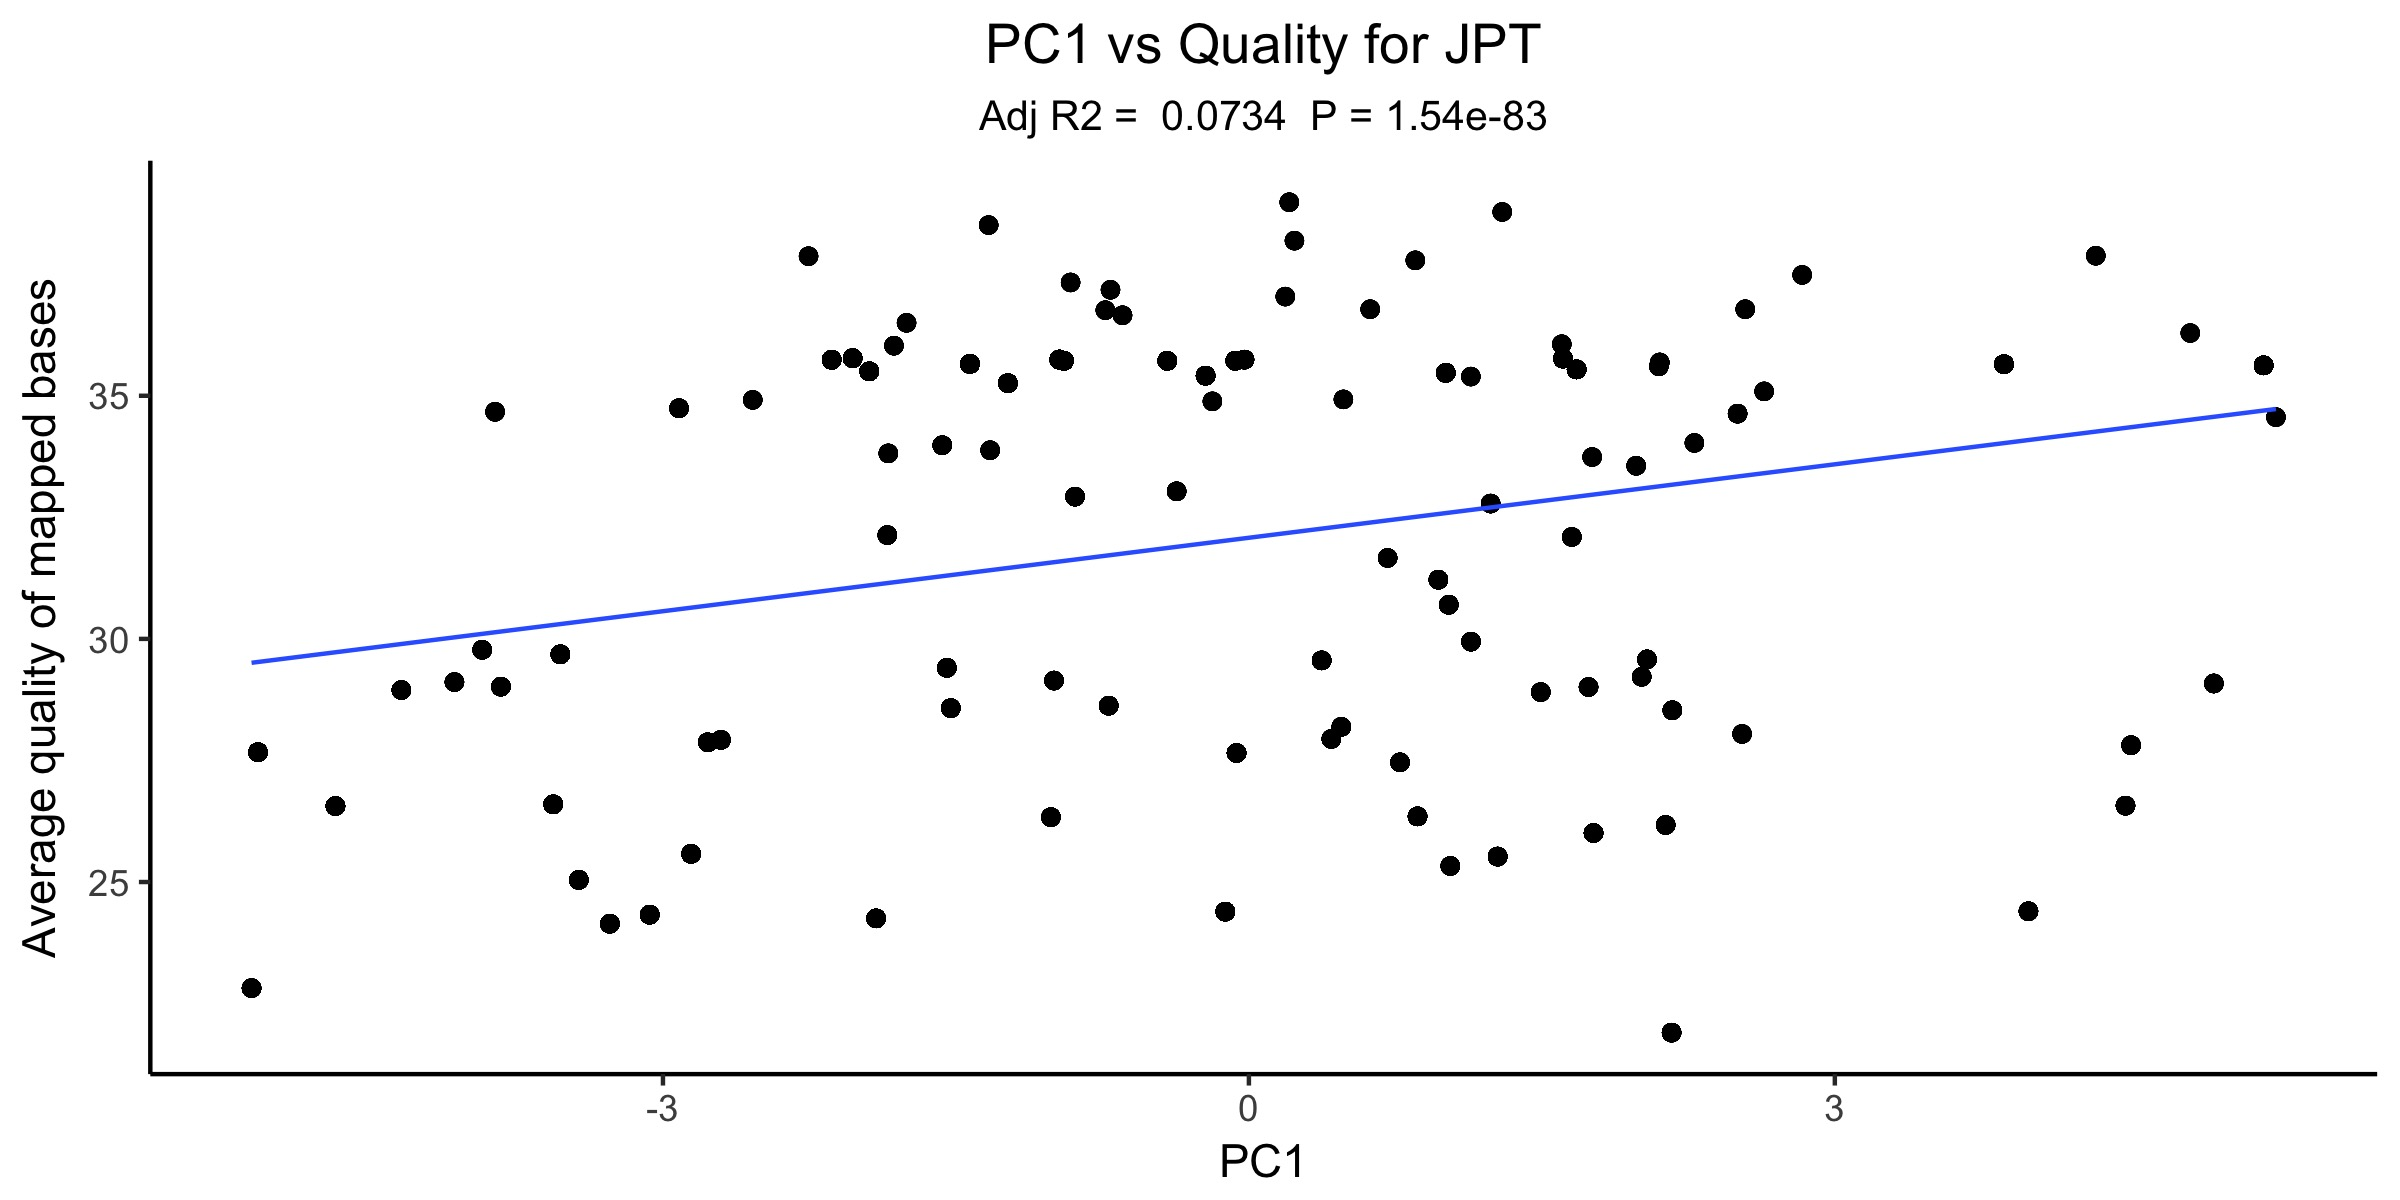
\includegraphics[width=\hsize,keepaspectratio]{./Figures/PC1_Correlation.jpg}
\caption{Regressions against the average quality per mapped bases $Q$ per individual is the best correlate with prevalence of the  *AC${\rightarrow}$*CC mutational signature in 1kGP, with individuals with low-quality data showing elevated rates of the signature.  }
\label{PC1_Correlation}
\end{figure}

\begin{figure}
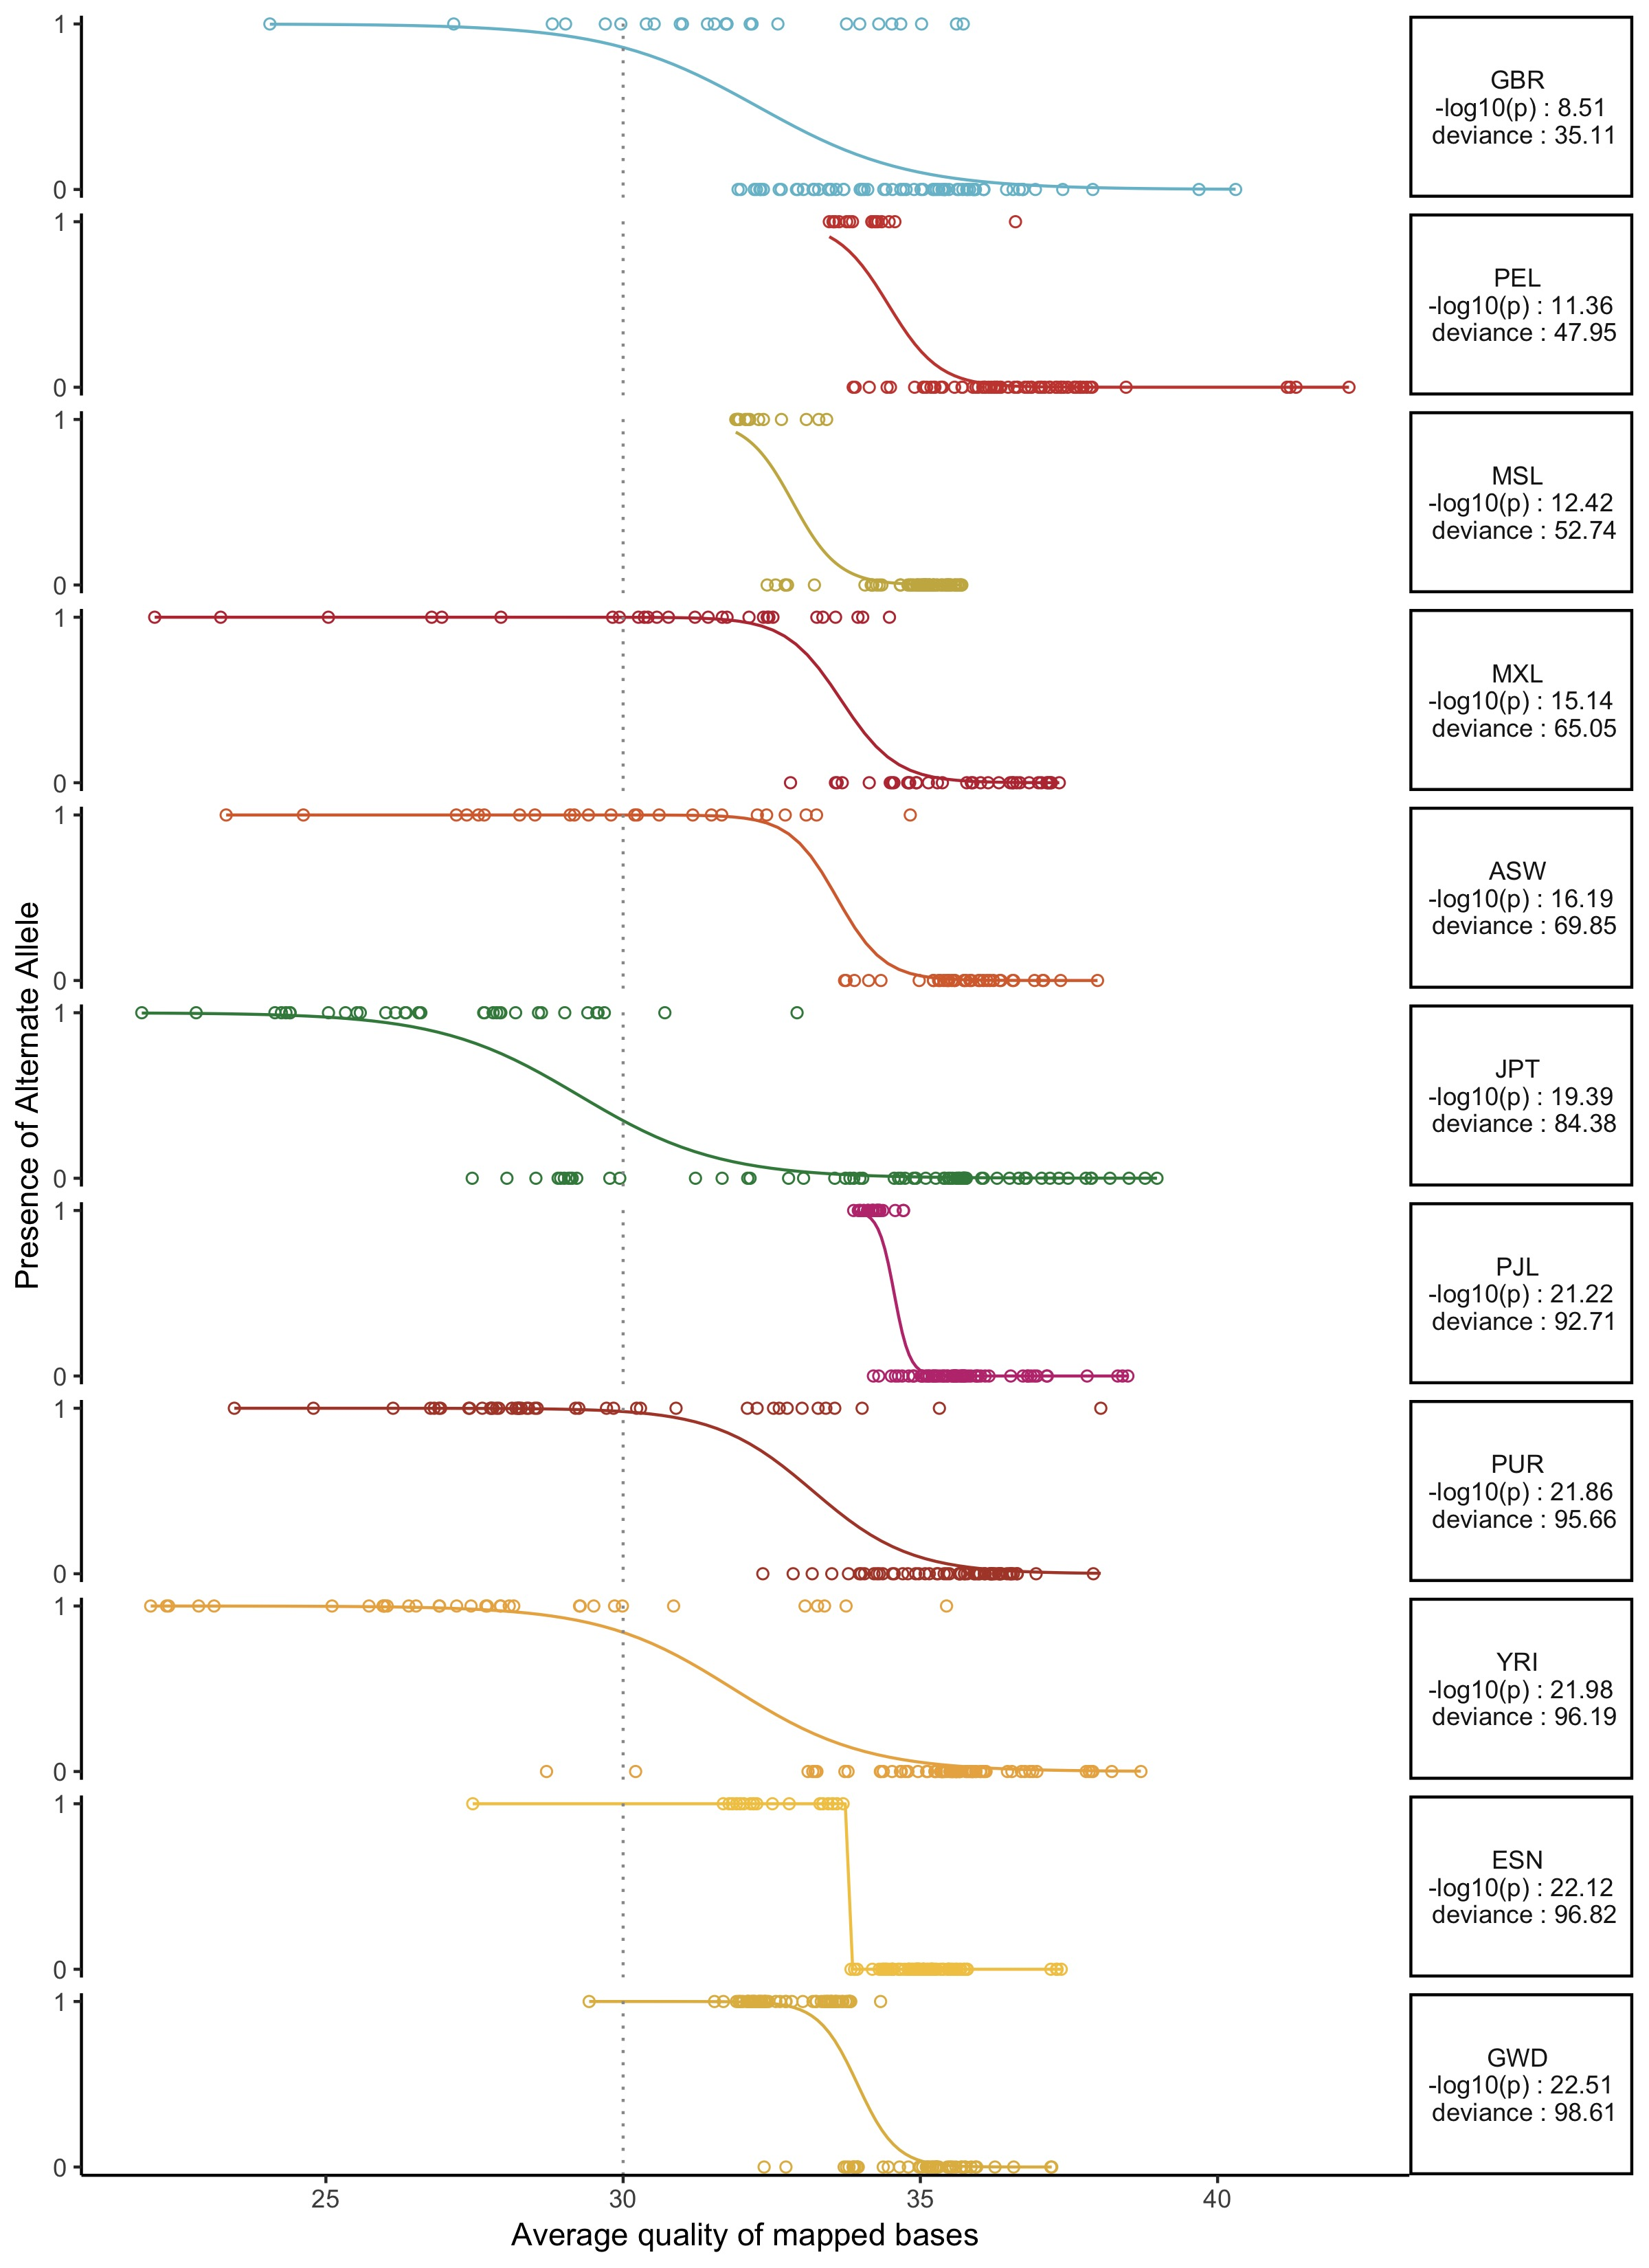
\includegraphics[width=\hsize,keepaspectratio]{./Figures/RegressionPlot_mostSig2.jpg}
\caption{Logistic regression of the most significantly associated SNP rs75254682 for the populations with significant association to the average quality per mapped bases $Q$.}
\label{MostSig}
\end{figure}

\begin{figure}
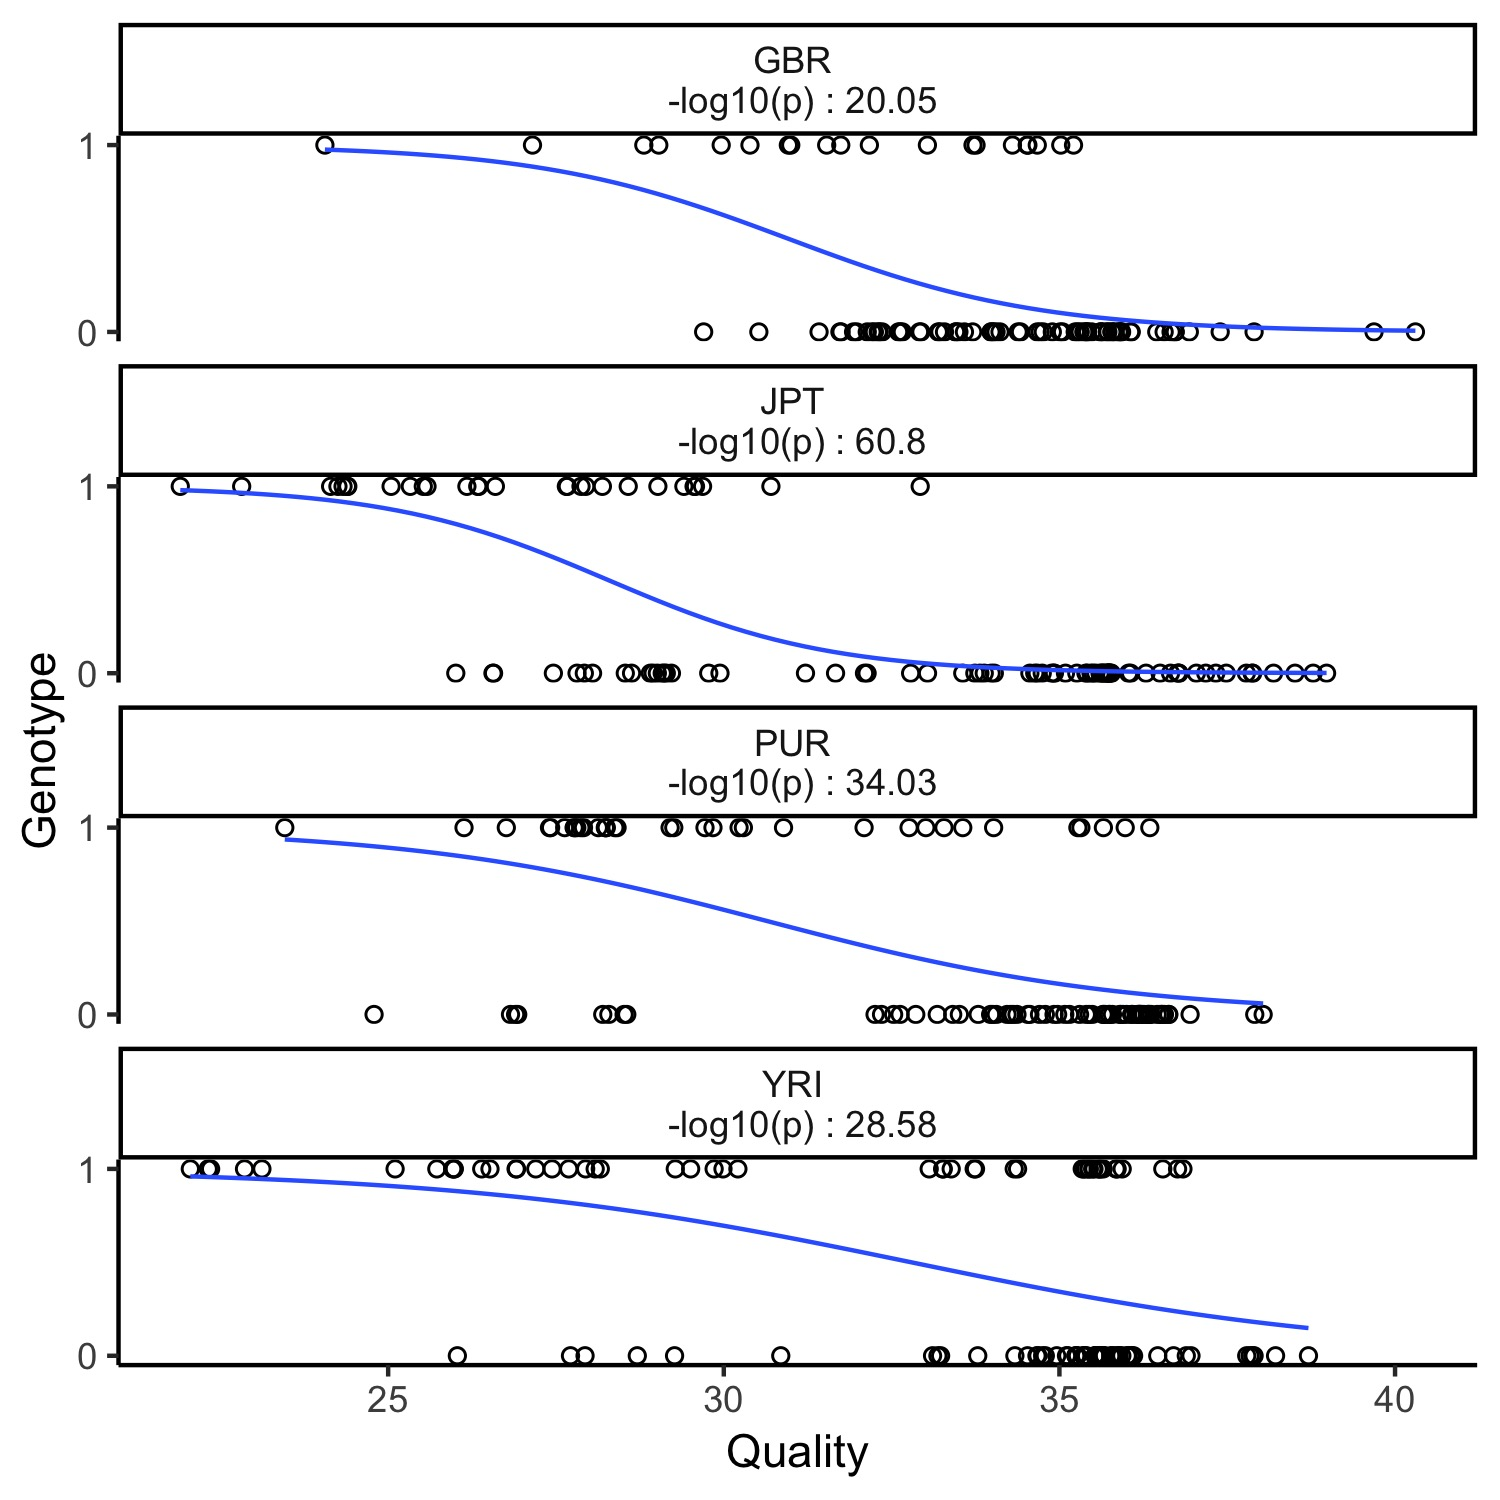
\includegraphics[width=\hsize,keepaspectratio]{./Figures/RegressionPlot.jpg}
\caption{Logistic regression of rs6057648 for the populations with significant association to the average quality per mapped bases $Q$.}
\label{TwinsSNP}
\end{figure}

\begin{figure}
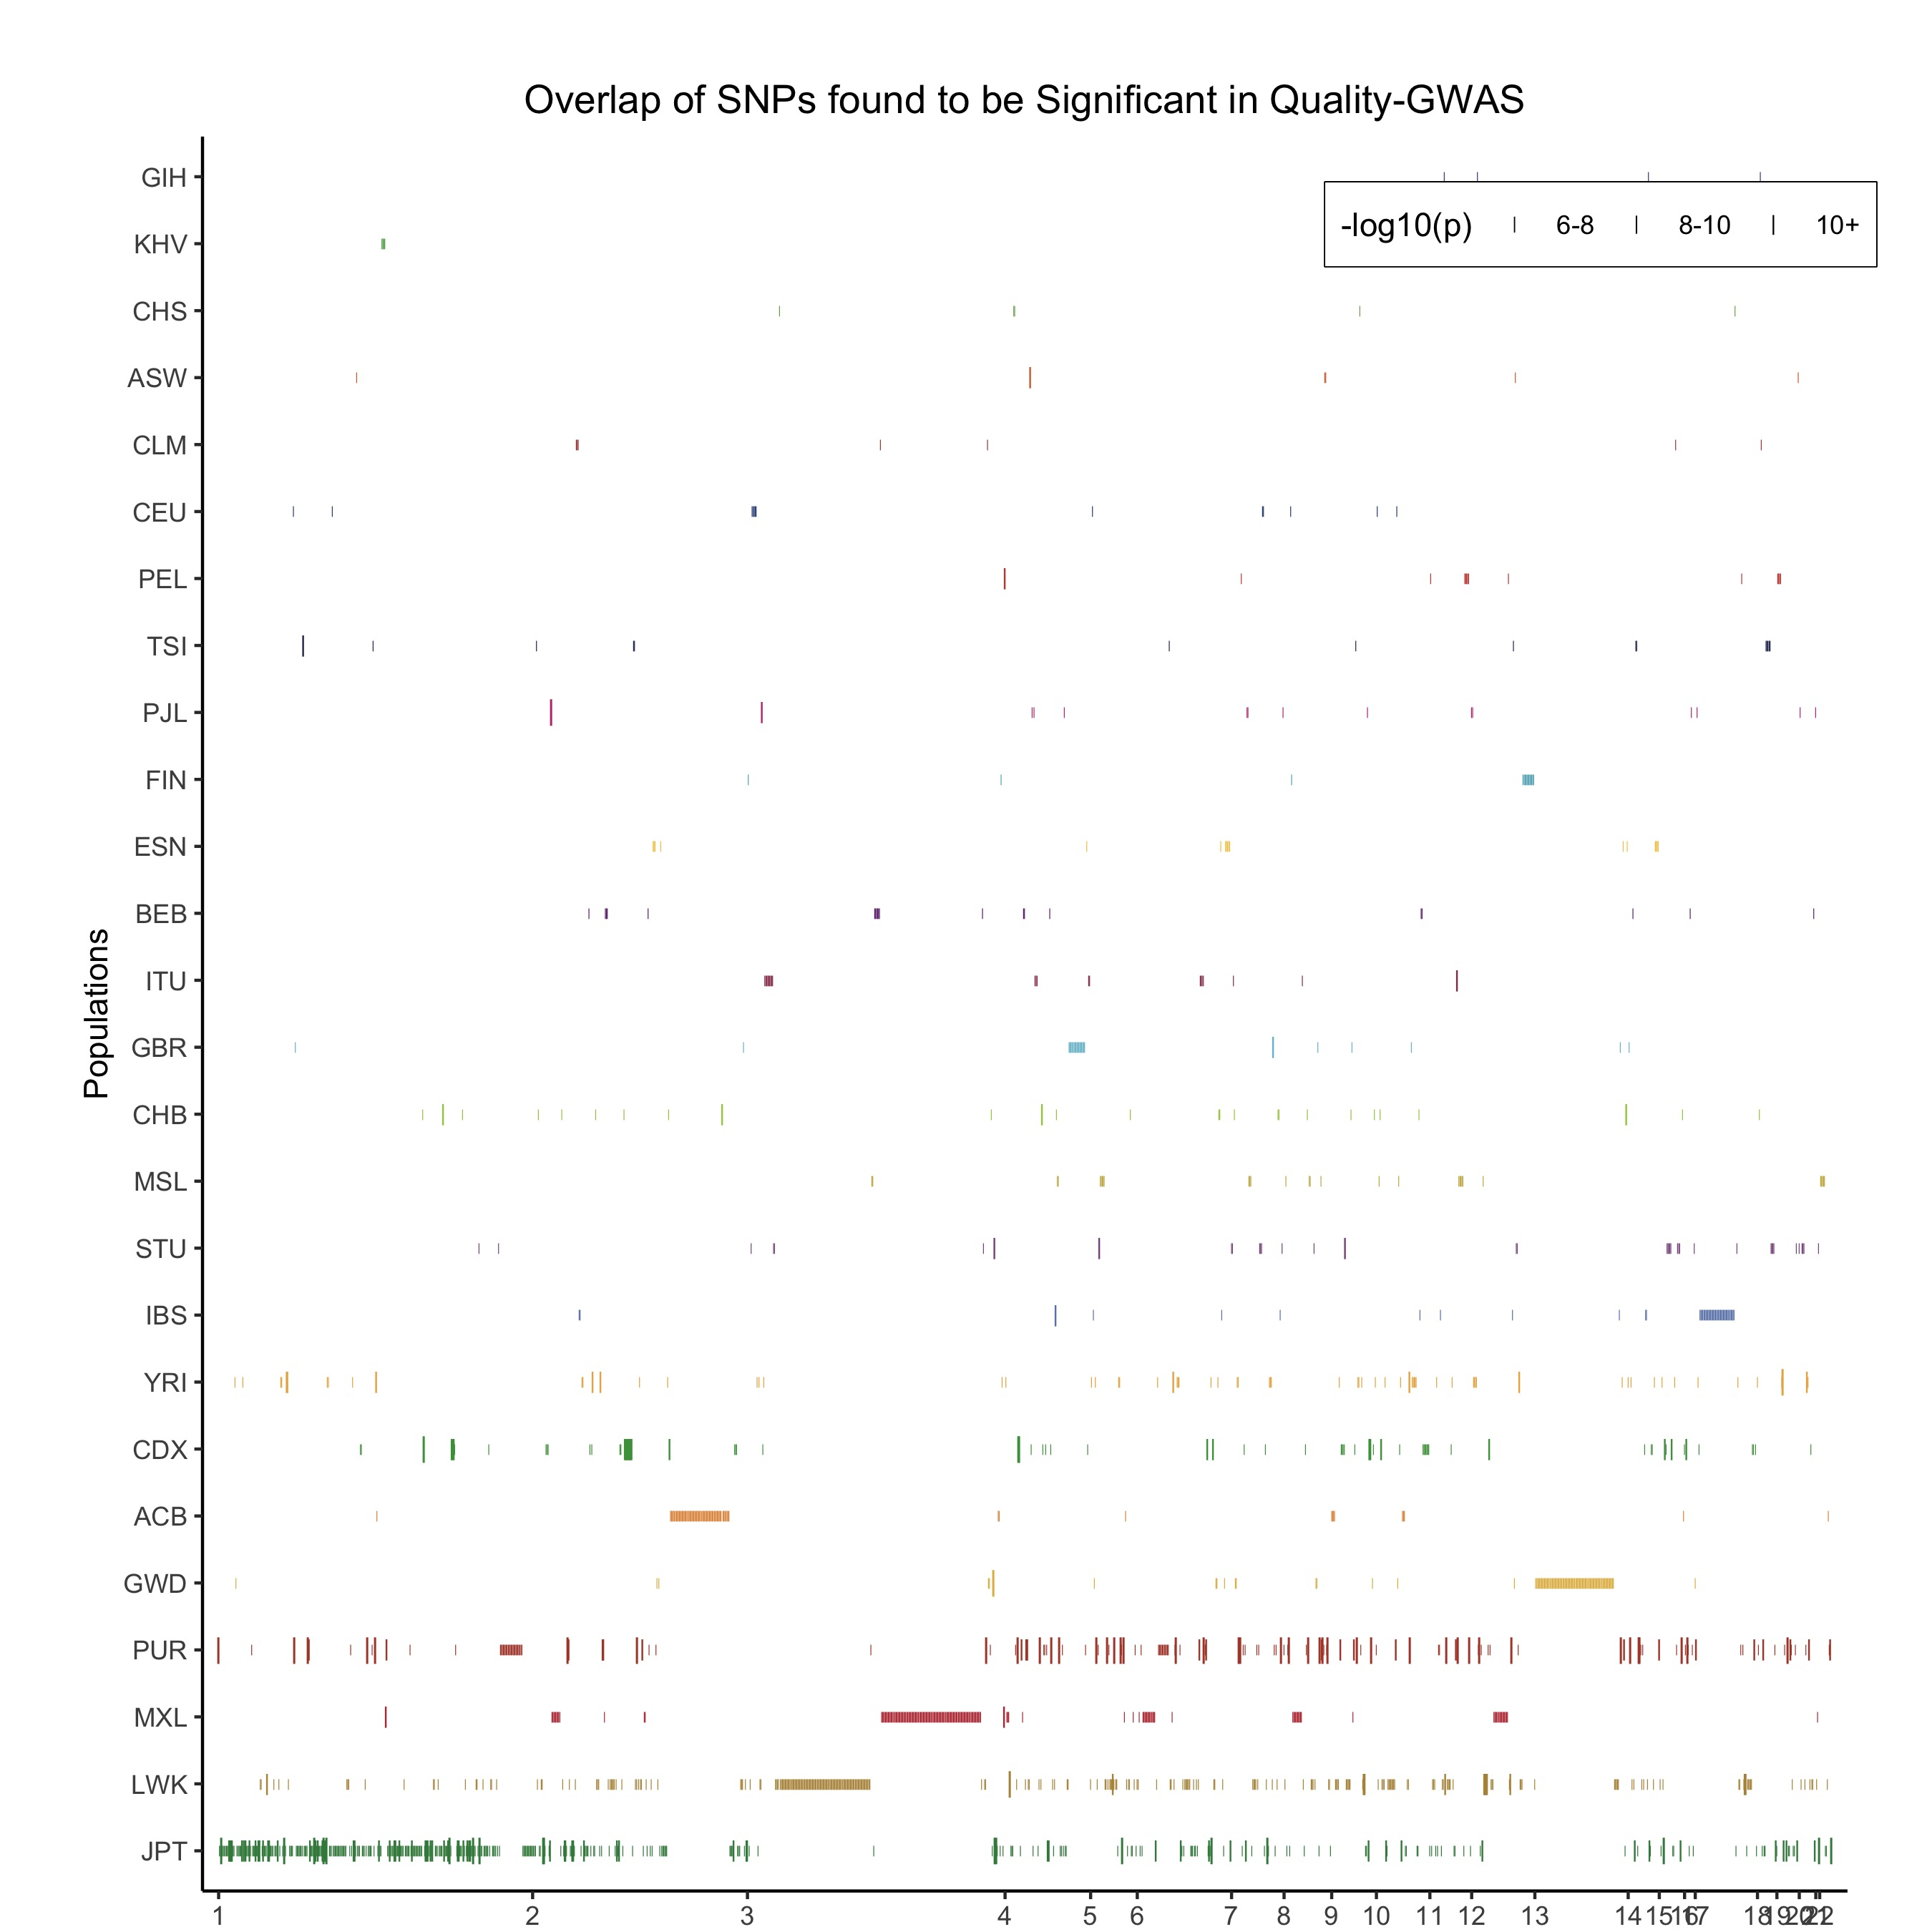
\includegraphics[width=\hsize,keepaspectratio]{./Figures/SNP6_Singles.jpg}
\caption{Significant SNPs found in only one population. The x-axis is sorted by genomic position.}
\label{Singles}
\end{figure}

\end{document}
			
%\begin{center}
 %\begin{tabular}{l l l r r} 
 %\hline
%Author & Year & Journal & RSID & PMID \\ [0.5ex] 
 %\hline
%Ebejer JL	& 2013	 & Twin Res Hum Genet & 	rs6057648&23527680\\ 
 
%Mandage R &	2017	 & PLoS One	 & rs200655768, rs184202621,&28654678\\
%& & & rs201255786, rs201761909&\\
%\hline
%\end{tabular}
%\end{center}